\documentclass[12pt]{article}
\usepackage[utf8]{inputenc}					%Inclui acentuação
\usepackage[brazil]{babel}					%Tradução de outputs para pt/br
\usepackage{indentfirst}					%Aplica identação nos primeiros parágrafos
\usepackage{setspace}						%Permite configurar espaçamentos
\usepackage[a4paper, margin=2cm]{geometry} 	%Altera a margem do documento
\usepackage[usenames, dvipnames]{xcolor}	%Modifica as cores
\usepackage{graphicx} 						%Permite adicionar figuras
\usepackage{float}							%Ajusta o posicionamento das figuras
\usepackage{multirow}						%Permite mesclar linhas de tabelas
\usepackage{tabularx}						%Ajuste de margem de tabelas
\usepackage{amsmath}						%Adiciona ferramentas ao ambiente matemático
\usepackage{natbib}							%Citações
\usepackage{physics}
\usepackage{amssymb}
\usepackage{mathtools}
\usepackage{listings,newtxtt}
\include{pgf}
\usepackage{natbib}
\lstset{basicstyle=\ttfamily, keywordstyle=\bfseries}



\setlength{\parindent}{1,5cm}				    %Altera a Identação
\onehalfspacing
\title{\textbf{\huge Projeto 1 - Física Computacional\\}Oscilador harmônico}
\author{Estevão Pimentel de Barcellos Santos}
\date{\today}


\begin{document}
    \null  % Empty line
    \nointerlineskip  % No skip for prev line
    \vfill
    \let\snewpage \newpage~
    \let\newpage \relax
    \maketitle
    \let \newpage \snewpage
    \vfill
    \thispagestyle{empty}
    \newpage
    \setcounter{page}{1}
    \section*{Resumo}
    Afim de explorar o cálculo numérico e os processos computacionais envolvidos na simulação de um oscilador
    harmônico foi construído, usando pyton, um simulador interativo de um pêndulo simples amortecido. Para
    a solução numérica foi experimentado o método de Euler, mas devido à sua perceptível imprecisão,
    especialmente para um oscilador harmônico em duas dimensões, foi substituído pelo método de Runge-Kutta.
    \section*{Oscilador harmônico}
    O que caracteriza um oscilador harmônico é que este pode ser descrito pela lei de Hooke.
    \begin{equation*}
        F(x) = -kx\;\;\;\;\leftrightarrow\;\;\;\;m\ddot{x} + kx=0
    \end{equation*}
    A solução dessa EDO é conhecida e pode ser expressa de duas formas
    \begin{equation*}
        \begin{aligned}
            x(t)&=A\sin(\omega_0t-\delta)\\
            x(t)&=A\cos(\omega_0t-\phi)
        \end{aligned}
    \end{equation*}
    em que $\omega_0=\sqrt{k/m}$. Isso para um oscilador harmônico unidimensional. A solução que nos interessa
    para o problema em questão é a do oscilador em duas dimensões, que de forma análoga é da da por
    \begin{equation*}
        \begin{aligned}
            x(t)&=A\sin(\omega_0t-\alpha)\\
            y(t)&=B\cos(\omega_0t-\beta)
        \end{aligned}
    \end{equation*}
    A equação diferencial que descreve um oscilador harmônico amortecido, difere por um termo de força resistiva
    $-b\dot{x}$.
    \begin{equation*}
            m\ddot{x}+b\dot{x}+kx=0
    \end{equation*}
    Cuja solução é dada por
    \begin{equation*}
        x(t)=e^{-\beta t}\left[A_1\exp\left(\sqrt{\beta^2-\omega_0^2}t\right)+A_2\exp\left(-\sqrt{\beta^2-\omega_0^2}t\right)\right]
    \end{equation*}
    Em que $\beta=b/2m$.
    \\Nesta solução, existem três casos gerais de interesse:
    \begin{table}[h]
        \begin{tabular}{llc}
        Subamortecimento:      & $\;\;\;\;\;\;\;\;\;\;\;\;\;\;\;\;\;\;\;\;\;\;\;\;\;\;$ & $\omega_0^2>\beta^2$ \\
        Amortecimento crítico: & $\;\;\;\;\;\;\;\;\;\;\;\;\;\;\;\;\;\;\;\;\;\;\;\;\;\;$ & $\omega_0^2=\beta^2$ \\
        Sobreamortecimento:    & $\;\;\;\;\;\;\;\;\;\;\;\;\;\;\;\;\;\;\;\;\;\;\;\;\;\;$ & $\omega_0^2<\beta^2$
        \end{tabular}
        \end{table}\\
    Os quais buscaremos explorar em nosso modelo mais adiante.
    \section*{Pêndulo simples}
    Podemos descrever um pêndulo simples a partir das forças que atuam sobre ele, isto é, o peso e
    a tensão do cabo. A tensão ata na direção radial ao movimento, enquanto o peso atua na vertical.
    Decompondo a tração em suas componentes horizontal e considerando o ponto mais baixo do arco como 
    formando um ângulo $\theta = 0$ com o eixo do pêndulo temos que
    \begin{equation*}
        \begin{aligned}
            &T_x = T\cos\theta\\
            &T_y = T\sin\theta
        \end{aligned}
    \end{equation*}
    As forças resultantes na vertical e na horizontal são, portanto, 
    \begin{equation*}
        \begin{aligned}
            &F_x = T\cos\theta\\
            &F_y = T\sin\theta + P
        \end{aligned}
    \end{equation*}
    em que $P$ é a força peso exercida sobre a carga do pêndulo. A tração é dada por
    \begin{equation*}
        T = \frac{mv^2}{L} + P\cos\theta
    \end{equation*}
    em que $m$ é a massa da carga, $v$ é sua velocidade, que é dada por $v = \sqrt{(v_x^2 + v_y^2)}$,
    e $L$ é o comprimento do cabo. Portanto as forças nos sentidos vertical e horizontal ficam
    \begin{equation*}
        \begin{aligned}
            &F_x = \left(\frac{mv^2}{L} + P\cos\theta\right)\cos\theta\\
            &F_y = \left(\frac{mv^2}{L} + P\cos\theta\right)\sin\theta + P
        \end{aligned}
    \end{equation*}
    Adicionando os termos de arraste $bv_x$ e $bv_y$ ficamos com
    \begin{equation*}
        \begin{aligned}
            &F_x = \left(\frac{mv^2}{L} + P\cos\theta\right)\cos\theta + bv_x\\
            &F_y = \left(\frac{mv^2}{L} + P\cos\theta\right)\sin\theta + P + bv_y
        \end{aligned}
    \end{equation*}
    Com isso e conhecidas as condições iniciais podemos aproximar o estado deste sistema para qualquer instante de 
    tempo usando calculo numérico iterando com pequenas variações de tempo.
    \newpage
    \section*{Método de Euler}
    O método de Euler é um procedimento numérico de pirmeira ordem que consiste
    na simples discretização da variável independente e na aproximação da função
    para uma composição de pontos que correspondem aos incrementos
    calculados dentro dos intervalos de tempo $\Delta t$ como mostra a figura a seguir.
    \begin{figure}[h]
        \centering
        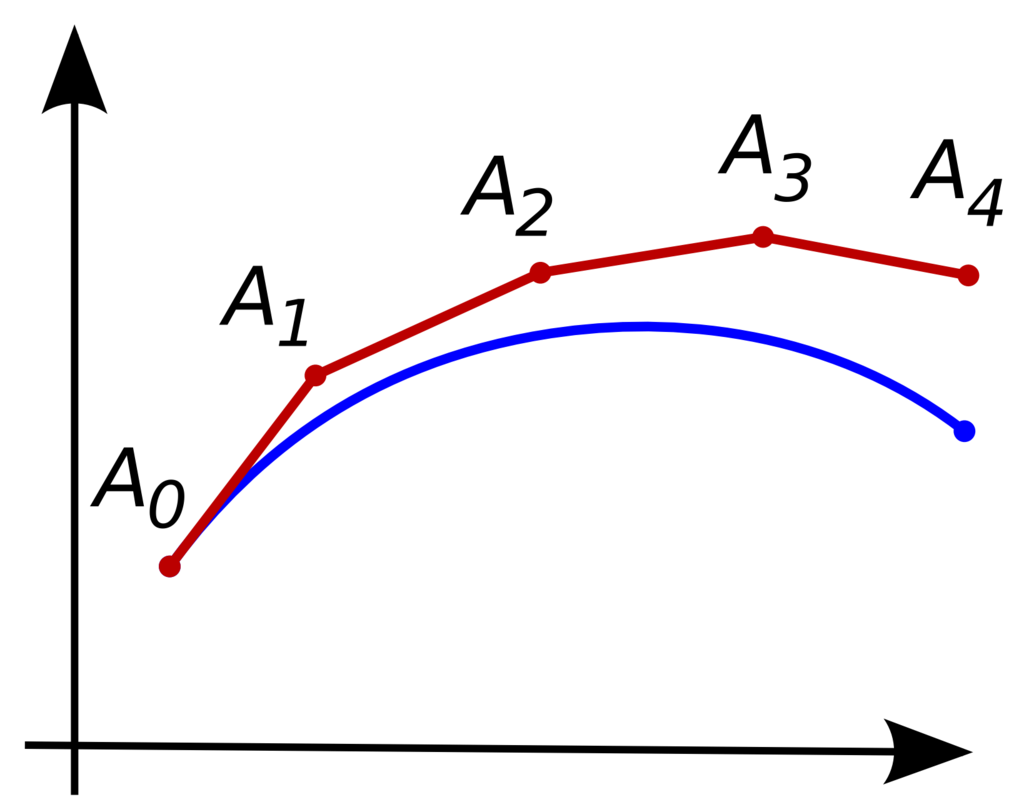
\includegraphics[scale=0.3]{1024px-Euler_method.png}
        \caption{Ilustração do método de Euler. A curva desconhecida está em azul, e sua aproximação polinomial está em vermelho.}
    \end{figure} 
    \par A precisão do método de Euler é perfeita para soluções lineares mas, como sugere a imagem
    é bastante grosseira para qualquer outro cenário. De fato, sempre podemos implementar o método
    de Euler com bastante precisão, basta reduzir suficientemente o tamanho de $\Delta t$ e
    alcançaremos a precisão desejada. O problema é que isso pode acabar tornando-se computacionalmente
    dispendioso até o ponto de se tornar inviável. Como ilustra a imagem, podemos perceber
    que os erros se acumulam com o tempo, o que pode tornar longas simulações simplesmente
    inviáveis, sendo preferível recorrer a outro algoritmo pra encontrar a solução.
    \par Para o problema do pêndulo, o método de Euler pode se mostrar razoável para pequenas
    oscilações e por um curto período de tempo. É possível estender o tempo e/ou o alcance de
    sua razoabilidade ao diminuir o tamanho de $\Delta t$ mas eventualmente o erro se tornará
    evidente.
    \par A fórmula recursiva do método de Euler para o problema do oscilador harmônico é dada por
    \begin{equation*}
        \boxed{
        \begin{aligned}
            x_{n+1}&=x_n+v_n\Delta t\\
            v_{n+1}&=v_n-\frac{k}{m}x_n\Delta t\\
            E_{n+1}&=\frac{1}{2}m\left(v_{n+1}\right)^2+\frac{1}{2}k(x_{n+1})^2
        \end{aligned}
        }
    \end{equation*}
    \section*{Método de Runge-Kutta}
    O método de Runge-Kutta difere do método de Euler por não ser um método de passo único, isto é, a cada iteração são 
    calculados passos intermediários para melhor estimar o próximo ponto.
    \begin{figure}[h]
        \centering
        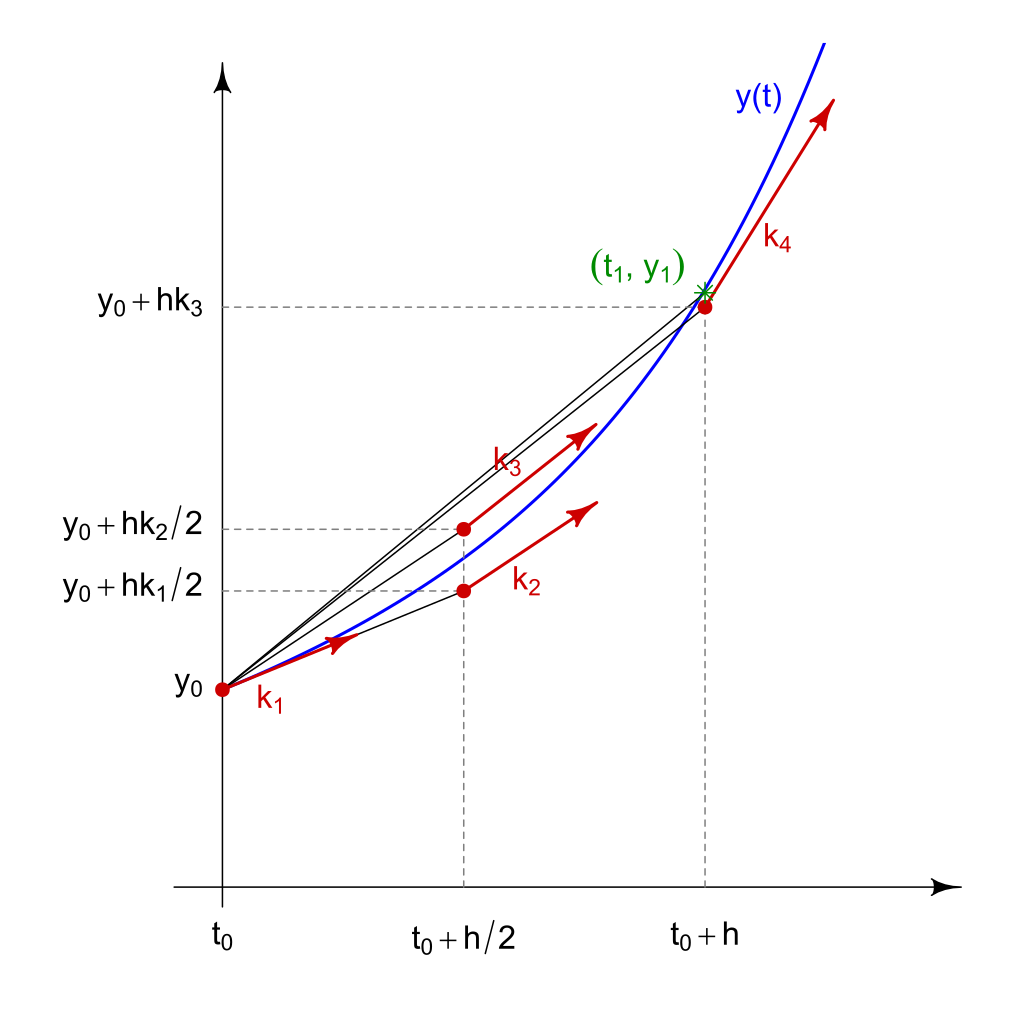
\includegraphics[scale=0.3]{1024px-Runge-Kutta_slopes.svg.png}
        \caption{Inclinações utilizadas pelo método de Runge-Kutta de quarta ordem.}
    \end{figure}
    \par Como é possível visualizar na figura acima, este método utiliza das derivadas calculadas nos passos intermediários
    para estimar a inclinação média do intervalo para então estimar o proximo ponto da curva. Para nosso modelo 
    implementaremos o método de Runge-Kutta de segunda ordem que utiliza apenas um passo intermediário e é exato para 
    soluções quadráticas, o que já o torna uma aproximação muitíssimo melhor que a do método de Euler.
    \par A fórmula recursiva do método de Runge-Kutta de segunda ordem para o problema do oscilador harmônico é dada por
    \begin{equation*}
        \begin{split}
            k_1^x&=v_n\Delta t\\
            k_1^v&=-(k/m)x_n\Delta t\\
            x_{1/2}&=x_n+k_1^x/2\\
            v_{1/2}&=v_n+k_1^v/2\\
            k_2^x&=v_{1/2}\Delta t\\
            k_2^v&=-(k/m)x_{1/2}\Delta t
        \end{split}
        \quad\quad\quad\quad\quad\quad
        \boxed{
        \begin{split}
            x_{n+1}&=x_n+k_2^x\\
            v_{n+1}&=v_n+k_2^v\\
            E_{n+1}&=\frac{1}{2}m\left(v_{n+1}\right)^2+\frac{1}{2}k\left(x_{n+1}\right)^2
        \end{split}
        }
    \end{equation*}
    \newpage
    \section*{Algoritmo}
    \noindent O algoritmo implementado no código reflete a seguinte sequência:\\\\
    Define-se a posição inicial $(x_0, y_0)$ e a massa da carga. A velocidade inicial é zero;\\\\
    Calcula-se o seno e o cosseno da atual posição em relação ao eixo do pêndulo: $\sin\theta = x_0/L$, $\cos\theta=y_0/L$;\\\\
    Calcula-se a força de tração exercida do cabo sobre a carga: $T=(mv^2)/L + mg\cos\theta$; \\\\
    Decompões-se a força do cabo em componentes vertical e horizontal, soma-se a componente vertical ao peso, soma-se ambas
    compontentes à sua respectiva força resistiva que será igual a uma constante multiplicada pela velocidade naquele eixo,
    e então calcula-se a aceleração da carga em ambos os eixos com $F=ma$;\\\\
    A partir da aceleração, calcula-se a velocidade num incremento de tempo $\Delta t/2$ com $V = V_0 + a\Delta t/2$
    e então calcula-se a posição deste ponto com $S = S_0 + v\Delta t/2$;\\\\
    De forma análoga aos processos anteriores, calcula-se neste novo ponto a velocidade e a aceleração nos eixos vertical e horizontal
    e estas serão usadas para calcular a posicição e a velocidade da carga no incremento de tempo $\Delta t$ a partir da posição e 
    da velocidade inicial.\\\\
    As novas posição e velocidade calculadas serão as condições iniciais da próxima iteração.\\\\
    Uma réplica do código pode ser vista na próxima página. As variáveis estão nomeadas de forma sugestiva para que seja
    compreensível.
    \newpage
\begin{lstlisting}[language=Python]
weight_pos = np.array([x0, y0])
delta_t = 1/60
Vx, Vy = 0, 0
mass_value = m
gravity_value = g
resistive_factor_value = r
while True:
    V0x, V0y = Vx, Vy
    sin_theta = (weight_pos[0]) / cable_lenght
    cos_theta = (weight_pos[1]) / cable_lenght
    T = ((mass_value * (Vx ** 2 + Vy ** 2))/(cable_lenght)) +\
        (mass_value * gravity_value * cos_theta)
    Fx = - T * sin_theta - resistive_factor_value * Vx
    Fy = - T * cos_theta + mass_value * gravity_value -\
        resistive_factor_value * Vy
    ax = Fx/mass_value
    ay = Fy/mass_value
    Vx_2 = (ax * (delta_t/2)) + Vx
    Vy_2 = (ay * (delta_t/2)) + Vy
    x_2 = weight_pos[0] + Vx * (delta_t/2)
    y_2 = weight_pos[1] + Vy * (delta_t/2)
    sin_theta_2 = (x_2) / cable_lenght
    cos_theta_2 = (y_2) / cable_lenght
    T_2 = ((mass_value * (Vx_2 ** 2 + Vy_2 ** 2))/\
         (cable_lenght)) + (mass_value * gravity_value *\
                            cos_theta_2)
    Fx_2 = - T_2 * sin_theta_2 - resistive_factor_value * Vx_2
    Fy_2 = - T_2 * cos_theta_2 + mass_value * gravity_value -\
          resistive_factor_value * Vy_2
    ax_2 = Fx_2/mass_value
    ay_2 = Fy_2/mass_value
    Vx = (ax_2 * (delta_t)) + V0x
    Vy = (ay_2 * (delta_t)) + V0y
    x = weight_pos[0] + Vx_2 * (delta_t)
    y = weight_pos[1] + Vy_2 * (delta_t)
    weight_pos = np.array([x, y])
\end{lstlisting}
    As variáveis  x0, y0, m, g e r representam valores arbitrários.
    \newpage
    \section*{Regimes de amortecimento}
    Para validar nosso modelo convém que avaliemos como ele se comporta no que diz respeito aos regímes de amortecimento.
    Considerando um pêndulo simples com uma carga de massa igual a $10\;kg$, um cabo com $10\;m$ de coprimento e uma aceleração
    gravitacional igual $10\;m/s^2$ e calculando o valor de $\beta$ obtemos que $\beta=4\;rad/s$ o que corresponde a um
    $b=2\;kg/s$.
    \par Fazendo testes com o simulador, é fácil perceber que com valores pequenos para o fator de arraste, isto é, para valores entre
    0 e 1, obtemos um regime semiamortecido. É característica do regime amortecido reduzir gradativamente a amplitude de oscilação
    ao longo de vários ciclos de oscilação de forma que com o tempo a amplitude tende a zero. Da mesma forma, para valores maiores
    ou iguais a 3 já é notório o regime de sobreamortecimento. Este regime é caracterizado por nenhuma oscilação e uma grande redução
    na velocidade de queda da carga do pêndulo. O amortecimento crítico por sua vez, é caracterizado pelo arreste mínimo em
    que não existe nenhuma oscilação, e ao fazer testes com o oscilador, variando progressivamente o fator de arraste em 0.1,
    o valor em que esse comportamento foi encontrado foi para um fator de arraste igual a 2, o que corresponde ao valor de $b$ previsto
    corroborando com a validade de nosso modelo.
    \begin{figure}[H]
        \centering
        \makebox[\textwidth]{\scalebox{0.4}{%% Creator: Matplotlib, PGF backend
%%
%% To include the figure in your LaTeX document, write
%%   \input{<filename>.pgf}
%%
%% Make sure the required packages are loaded in your preamble
%%   \usepackage{pgf}
%%
%% Figures using additional raster images can only be included by \input if
%% they are in the same directory as the main LaTeX file. For loading figures
%% from other directories you can use the `import` package
%%   \usepackage{import}
%%
%% and then include the figures with
%%   \import{<path to file>}{<filename>.pgf}
%%
%% Matplotlib used the following preamble
%%   \usepackage{fontspec}
%%   \setmainfont{DejaVuSerif.ttf}[Path=\detokenize{/home/estevao/Projetos/Projeto 1/venv/lib/python3.9/site-packages/matplotlib/mpl-data/fonts/ttf/}]
%%   \setsansfont{DejaVuSans.ttf}[Path=\detokenize{/home/estevao/Projetos/Projeto 1/venv/lib/python3.9/site-packages/matplotlib/mpl-data/fonts/ttf/}]
%%   \setmonofont{DejaVuSansMono.ttf}[Path=\detokenize{/home/estevao/Projetos/Projeto 1/venv/lib/python3.9/site-packages/matplotlib/mpl-data/fonts/ttf/}]
%%
\begingroup%
\makeatletter%
\begin{pgfpicture}%
\pgfpathrectangle{\pgfpointorigin}{\pgfqpoint{19.200000in}{9.740000in}}%
\pgfusepath{use as bounding box, clip}%
\begin{pgfscope}%
\pgfsetbuttcap%
\pgfsetmiterjoin%
\definecolor{currentfill}{rgb}{1.000000,1.000000,1.000000}%
\pgfsetfillcolor{currentfill}%
\pgfsetlinewidth{0.000000pt}%
\definecolor{currentstroke}{rgb}{1.000000,1.000000,1.000000}%
\pgfsetstrokecolor{currentstroke}%
\pgfsetdash{}{0pt}%
\pgfpathmoveto{\pgfqpoint{0.000000in}{0.000000in}}%
\pgfpathlineto{\pgfqpoint{19.200000in}{0.000000in}}%
\pgfpathlineto{\pgfqpoint{19.200000in}{9.740000in}}%
\pgfpathlineto{\pgfqpoint{0.000000in}{9.740000in}}%
\pgfpathclose%
\pgfusepath{fill}%
\end{pgfscope}%
\begin{pgfscope}%
\pgfsetbuttcap%
\pgfsetmiterjoin%
\definecolor{currentfill}{rgb}{1.000000,1.000000,1.000000}%
\pgfsetfillcolor{currentfill}%
\pgfsetlinewidth{0.000000pt}%
\definecolor{currentstroke}{rgb}{0.000000,0.000000,0.000000}%
\pgfsetstrokecolor{currentstroke}%
\pgfsetstrokeopacity{0.000000}%
\pgfsetdash{}{0pt}%
\pgfpathmoveto{\pgfqpoint{2.400000in}{1.071400in}}%
\pgfpathlineto{\pgfqpoint{17.280000in}{1.071400in}}%
\pgfpathlineto{\pgfqpoint{17.280000in}{8.571200in}}%
\pgfpathlineto{\pgfqpoint{2.400000in}{8.571200in}}%
\pgfpathclose%
\pgfusepath{fill}%
\end{pgfscope}%
\begin{pgfscope}%
\pgfsetbuttcap%
\pgfsetroundjoin%
\definecolor{currentfill}{rgb}{0.000000,0.000000,0.000000}%
\pgfsetfillcolor{currentfill}%
\pgfsetlinewidth{0.803000pt}%
\definecolor{currentstroke}{rgb}{0.000000,0.000000,0.000000}%
\pgfsetstrokecolor{currentstroke}%
\pgfsetdash{}{0pt}%
\pgfsys@defobject{currentmarker}{\pgfqpoint{0.000000in}{-0.048611in}}{\pgfqpoint{0.000000in}{0.000000in}}{%
\pgfpathmoveto{\pgfqpoint{0.000000in}{0.000000in}}%
\pgfpathlineto{\pgfqpoint{0.000000in}{-0.048611in}}%
\pgfusepath{stroke,fill}%
}%
\begin{pgfscope}%
\pgfsys@transformshift{3.076364in}{1.071400in}%
\pgfsys@useobject{currentmarker}{}%
\end{pgfscope}%
\end{pgfscope}%
\begin{pgfscope}%
\definecolor{textcolor}{rgb}{0.000000,0.000000,0.000000}%
\pgfsetstrokecolor{textcolor}%
\pgfsetfillcolor{textcolor}%
\pgftext[x=3.076364in,y=0.974178in,,top]{\color{textcolor}\sffamily\fontsize{30.000000}{36.000000}\selectfont 0}%
\end{pgfscope}%
\begin{pgfscope}%
\pgfsetbuttcap%
\pgfsetroundjoin%
\definecolor{currentfill}{rgb}{0.000000,0.000000,0.000000}%
\pgfsetfillcolor{currentfill}%
\pgfsetlinewidth{0.803000pt}%
\definecolor{currentstroke}{rgb}{0.000000,0.000000,0.000000}%
\pgfsetstrokecolor{currentstroke}%
\pgfsetdash{}{0pt}%
\pgfsys@defobject{currentmarker}{\pgfqpoint{0.000000in}{-0.048611in}}{\pgfqpoint{0.000000in}{0.000000in}}{%
\pgfpathmoveto{\pgfqpoint{0.000000in}{0.000000in}}%
\pgfpathlineto{\pgfqpoint{0.000000in}{-0.048611in}}%
\pgfusepath{stroke,fill}%
}%
\begin{pgfscope}%
\pgfsys@transformshift{5.781818in}{1.071400in}%
\pgfsys@useobject{currentmarker}{}%
\end{pgfscope}%
\end{pgfscope}%
\begin{pgfscope}%
\definecolor{textcolor}{rgb}{0.000000,0.000000,0.000000}%
\pgfsetstrokecolor{textcolor}%
\pgfsetfillcolor{textcolor}%
\pgftext[x=5.781818in,y=0.974178in,,top]{\color{textcolor}\sffamily\fontsize{30.000000}{36.000000}\selectfont 2}%
\end{pgfscope}%
\begin{pgfscope}%
\pgfsetbuttcap%
\pgfsetroundjoin%
\definecolor{currentfill}{rgb}{0.000000,0.000000,0.000000}%
\pgfsetfillcolor{currentfill}%
\pgfsetlinewidth{0.803000pt}%
\definecolor{currentstroke}{rgb}{0.000000,0.000000,0.000000}%
\pgfsetstrokecolor{currentstroke}%
\pgfsetdash{}{0pt}%
\pgfsys@defobject{currentmarker}{\pgfqpoint{0.000000in}{-0.048611in}}{\pgfqpoint{0.000000in}{0.000000in}}{%
\pgfpathmoveto{\pgfqpoint{0.000000in}{0.000000in}}%
\pgfpathlineto{\pgfqpoint{0.000000in}{-0.048611in}}%
\pgfusepath{stroke,fill}%
}%
\begin{pgfscope}%
\pgfsys@transformshift{8.487273in}{1.071400in}%
\pgfsys@useobject{currentmarker}{}%
\end{pgfscope}%
\end{pgfscope}%
\begin{pgfscope}%
\definecolor{textcolor}{rgb}{0.000000,0.000000,0.000000}%
\pgfsetstrokecolor{textcolor}%
\pgfsetfillcolor{textcolor}%
\pgftext[x=8.487273in,y=0.974178in,,top]{\color{textcolor}\sffamily\fontsize{30.000000}{36.000000}\selectfont 4}%
\end{pgfscope}%
\begin{pgfscope}%
\pgfsetbuttcap%
\pgfsetroundjoin%
\definecolor{currentfill}{rgb}{0.000000,0.000000,0.000000}%
\pgfsetfillcolor{currentfill}%
\pgfsetlinewidth{0.803000pt}%
\definecolor{currentstroke}{rgb}{0.000000,0.000000,0.000000}%
\pgfsetstrokecolor{currentstroke}%
\pgfsetdash{}{0pt}%
\pgfsys@defobject{currentmarker}{\pgfqpoint{0.000000in}{-0.048611in}}{\pgfqpoint{0.000000in}{0.000000in}}{%
\pgfpathmoveto{\pgfqpoint{0.000000in}{0.000000in}}%
\pgfpathlineto{\pgfqpoint{0.000000in}{-0.048611in}}%
\pgfusepath{stroke,fill}%
}%
\begin{pgfscope}%
\pgfsys@transformshift{11.192727in}{1.071400in}%
\pgfsys@useobject{currentmarker}{}%
\end{pgfscope}%
\end{pgfscope}%
\begin{pgfscope}%
\definecolor{textcolor}{rgb}{0.000000,0.000000,0.000000}%
\pgfsetstrokecolor{textcolor}%
\pgfsetfillcolor{textcolor}%
\pgftext[x=11.192727in,y=0.974178in,,top]{\color{textcolor}\sffamily\fontsize{30.000000}{36.000000}\selectfont 6}%
\end{pgfscope}%
\begin{pgfscope}%
\pgfsetbuttcap%
\pgfsetroundjoin%
\definecolor{currentfill}{rgb}{0.000000,0.000000,0.000000}%
\pgfsetfillcolor{currentfill}%
\pgfsetlinewidth{0.803000pt}%
\definecolor{currentstroke}{rgb}{0.000000,0.000000,0.000000}%
\pgfsetstrokecolor{currentstroke}%
\pgfsetdash{}{0pt}%
\pgfsys@defobject{currentmarker}{\pgfqpoint{0.000000in}{-0.048611in}}{\pgfqpoint{0.000000in}{0.000000in}}{%
\pgfpathmoveto{\pgfqpoint{0.000000in}{0.000000in}}%
\pgfpathlineto{\pgfqpoint{0.000000in}{-0.048611in}}%
\pgfusepath{stroke,fill}%
}%
\begin{pgfscope}%
\pgfsys@transformshift{13.898182in}{1.071400in}%
\pgfsys@useobject{currentmarker}{}%
\end{pgfscope}%
\end{pgfscope}%
\begin{pgfscope}%
\definecolor{textcolor}{rgb}{0.000000,0.000000,0.000000}%
\pgfsetstrokecolor{textcolor}%
\pgfsetfillcolor{textcolor}%
\pgftext[x=13.898182in,y=0.974178in,,top]{\color{textcolor}\sffamily\fontsize{30.000000}{36.000000}\selectfont 8}%
\end{pgfscope}%
\begin{pgfscope}%
\pgfsetbuttcap%
\pgfsetroundjoin%
\definecolor{currentfill}{rgb}{0.000000,0.000000,0.000000}%
\pgfsetfillcolor{currentfill}%
\pgfsetlinewidth{0.803000pt}%
\definecolor{currentstroke}{rgb}{0.000000,0.000000,0.000000}%
\pgfsetstrokecolor{currentstroke}%
\pgfsetdash{}{0pt}%
\pgfsys@defobject{currentmarker}{\pgfqpoint{0.000000in}{-0.048611in}}{\pgfqpoint{0.000000in}{0.000000in}}{%
\pgfpathmoveto{\pgfqpoint{0.000000in}{0.000000in}}%
\pgfpathlineto{\pgfqpoint{0.000000in}{-0.048611in}}%
\pgfusepath{stroke,fill}%
}%
\begin{pgfscope}%
\pgfsys@transformshift{16.603636in}{1.071400in}%
\pgfsys@useobject{currentmarker}{}%
\end{pgfscope}%
\end{pgfscope}%
\begin{pgfscope}%
\definecolor{textcolor}{rgb}{0.000000,0.000000,0.000000}%
\pgfsetstrokecolor{textcolor}%
\pgfsetfillcolor{textcolor}%
\pgftext[x=16.603636in,y=0.974178in,,top]{\color{textcolor}\sffamily\fontsize{30.000000}{36.000000}\selectfont 10}%
\end{pgfscope}%
\begin{pgfscope}%
\definecolor{textcolor}{rgb}{0.000000,0.000000,0.000000}%
\pgfsetstrokecolor{textcolor}%
\pgfsetfillcolor{textcolor}%
\pgftext[x=9.840000in,y=0.515383in,,top]{\color{textcolor}\sffamily\fontsize{30.000000}{36.000000}\selectfont Tempo (s)}%
\end{pgfscope}%
\begin{pgfscope}%
\pgfsetbuttcap%
\pgfsetroundjoin%
\definecolor{currentfill}{rgb}{0.000000,0.000000,0.000000}%
\pgfsetfillcolor{currentfill}%
\pgfsetlinewidth{0.803000pt}%
\definecolor{currentstroke}{rgb}{0.000000,0.000000,0.000000}%
\pgfsetstrokecolor{currentstroke}%
\pgfsetdash{}{0pt}%
\pgfsys@defobject{currentmarker}{\pgfqpoint{-0.048611in}{0.000000in}}{\pgfqpoint{-0.000000in}{0.000000in}}{%
\pgfpathmoveto{\pgfqpoint{-0.000000in}{0.000000in}}%
\pgfpathlineto{\pgfqpoint{-0.048611in}{0.000000in}}%
\pgfusepath{stroke,fill}%
}%
\begin{pgfscope}%
\pgfsys@transformshift{2.400000in}{1.412293in}%
\pgfsys@useobject{currentmarker}{}%
\end{pgfscope}%
\end{pgfscope}%
\begin{pgfscope}%
\definecolor{textcolor}{rgb}{0.000000,0.000000,0.000000}%
\pgfsetstrokecolor{textcolor}%
\pgfsetfillcolor{textcolor}%
\pgftext[x=2.037682in, y=1.254008in, left, base]{\color{textcolor}\sffamily\fontsize{30.000000}{36.000000}\selectfont 0}%
\end{pgfscope}%
\begin{pgfscope}%
\pgfsetbuttcap%
\pgfsetroundjoin%
\definecolor{currentfill}{rgb}{0.000000,0.000000,0.000000}%
\pgfsetfillcolor{currentfill}%
\pgfsetlinewidth{0.803000pt}%
\definecolor{currentstroke}{rgb}{0.000000,0.000000,0.000000}%
\pgfsetstrokecolor{currentstroke}%
\pgfsetdash{}{0pt}%
\pgfsys@defobject{currentmarker}{\pgfqpoint{-0.048611in}{0.000000in}}{\pgfqpoint{-0.000000in}{0.000000in}}{%
\pgfpathmoveto{\pgfqpoint{-0.000000in}{0.000000in}}%
\pgfpathlineto{\pgfqpoint{-0.048611in}{0.000000in}}%
\pgfusepath{stroke,fill}%
}%
\begin{pgfscope}%
\pgfsys@transformshift{2.400000in}{2.776370in}%
\pgfsys@useobject{currentmarker}{}%
\end{pgfscope}%
\end{pgfscope}%
\begin{pgfscope}%
\definecolor{textcolor}{rgb}{0.000000,0.000000,0.000000}%
\pgfsetstrokecolor{textcolor}%
\pgfsetfillcolor{textcolor}%
\pgftext[x=1.772586in, y=2.618086in, left, base]{\color{textcolor}\sffamily\fontsize{30.000000}{36.000000}\selectfont 20}%
\end{pgfscope}%
\begin{pgfscope}%
\pgfsetbuttcap%
\pgfsetroundjoin%
\definecolor{currentfill}{rgb}{0.000000,0.000000,0.000000}%
\pgfsetfillcolor{currentfill}%
\pgfsetlinewidth{0.803000pt}%
\definecolor{currentstroke}{rgb}{0.000000,0.000000,0.000000}%
\pgfsetstrokecolor{currentstroke}%
\pgfsetdash{}{0pt}%
\pgfsys@defobject{currentmarker}{\pgfqpoint{-0.048611in}{0.000000in}}{\pgfqpoint{-0.000000in}{0.000000in}}{%
\pgfpathmoveto{\pgfqpoint{-0.000000in}{0.000000in}}%
\pgfpathlineto{\pgfqpoint{-0.048611in}{0.000000in}}%
\pgfusepath{stroke,fill}%
}%
\begin{pgfscope}%
\pgfsys@transformshift{2.400000in}{4.140447in}%
\pgfsys@useobject{currentmarker}{}%
\end{pgfscope}%
\end{pgfscope}%
\begin{pgfscope}%
\definecolor{textcolor}{rgb}{0.000000,0.000000,0.000000}%
\pgfsetstrokecolor{textcolor}%
\pgfsetfillcolor{textcolor}%
\pgftext[x=1.772586in, y=3.982163in, left, base]{\color{textcolor}\sffamily\fontsize{30.000000}{36.000000}\selectfont 40}%
\end{pgfscope}%
\begin{pgfscope}%
\pgfsetbuttcap%
\pgfsetroundjoin%
\definecolor{currentfill}{rgb}{0.000000,0.000000,0.000000}%
\pgfsetfillcolor{currentfill}%
\pgfsetlinewidth{0.803000pt}%
\definecolor{currentstroke}{rgb}{0.000000,0.000000,0.000000}%
\pgfsetstrokecolor{currentstroke}%
\pgfsetdash{}{0pt}%
\pgfsys@defobject{currentmarker}{\pgfqpoint{-0.048611in}{0.000000in}}{\pgfqpoint{-0.000000in}{0.000000in}}{%
\pgfpathmoveto{\pgfqpoint{-0.000000in}{0.000000in}}%
\pgfpathlineto{\pgfqpoint{-0.048611in}{0.000000in}}%
\pgfusepath{stroke,fill}%
}%
\begin{pgfscope}%
\pgfsys@transformshift{2.400000in}{5.504525in}%
\pgfsys@useobject{currentmarker}{}%
\end{pgfscope}%
\end{pgfscope}%
\begin{pgfscope}%
\definecolor{textcolor}{rgb}{0.000000,0.000000,0.000000}%
\pgfsetstrokecolor{textcolor}%
\pgfsetfillcolor{textcolor}%
\pgftext[x=1.772586in, y=5.346240in, left, base]{\color{textcolor}\sffamily\fontsize{30.000000}{36.000000}\selectfont 60}%
\end{pgfscope}%
\begin{pgfscope}%
\pgfsetbuttcap%
\pgfsetroundjoin%
\definecolor{currentfill}{rgb}{0.000000,0.000000,0.000000}%
\pgfsetfillcolor{currentfill}%
\pgfsetlinewidth{0.803000pt}%
\definecolor{currentstroke}{rgb}{0.000000,0.000000,0.000000}%
\pgfsetstrokecolor{currentstroke}%
\pgfsetdash{}{0pt}%
\pgfsys@defobject{currentmarker}{\pgfqpoint{-0.048611in}{0.000000in}}{\pgfqpoint{-0.000000in}{0.000000in}}{%
\pgfpathmoveto{\pgfqpoint{-0.000000in}{0.000000in}}%
\pgfpathlineto{\pgfqpoint{-0.048611in}{0.000000in}}%
\pgfusepath{stroke,fill}%
}%
\begin{pgfscope}%
\pgfsys@transformshift{2.400000in}{6.868602in}%
\pgfsys@useobject{currentmarker}{}%
\end{pgfscope}%
\end{pgfscope}%
\begin{pgfscope}%
\definecolor{textcolor}{rgb}{0.000000,0.000000,0.000000}%
\pgfsetstrokecolor{textcolor}%
\pgfsetfillcolor{textcolor}%
\pgftext[x=1.772586in, y=6.710317in, left, base]{\color{textcolor}\sffamily\fontsize{30.000000}{36.000000}\selectfont 80}%
\end{pgfscope}%
\begin{pgfscope}%
\pgfsetbuttcap%
\pgfsetroundjoin%
\definecolor{currentfill}{rgb}{0.000000,0.000000,0.000000}%
\pgfsetfillcolor{currentfill}%
\pgfsetlinewidth{0.803000pt}%
\definecolor{currentstroke}{rgb}{0.000000,0.000000,0.000000}%
\pgfsetstrokecolor{currentstroke}%
\pgfsetdash{}{0pt}%
\pgfsys@defobject{currentmarker}{\pgfqpoint{-0.048611in}{0.000000in}}{\pgfqpoint{-0.000000in}{0.000000in}}{%
\pgfpathmoveto{\pgfqpoint{-0.000000in}{0.000000in}}%
\pgfpathlineto{\pgfqpoint{-0.048611in}{0.000000in}}%
\pgfusepath{stroke,fill}%
}%
\begin{pgfscope}%
\pgfsys@transformshift{2.400000in}{8.232679in}%
\pgfsys@useobject{currentmarker}{}%
\end{pgfscope}%
\end{pgfscope}%
\begin{pgfscope}%
\definecolor{textcolor}{rgb}{0.000000,0.000000,0.000000}%
\pgfsetstrokecolor{textcolor}%
\pgfsetfillcolor{textcolor}%
\pgftext[x=1.507490in, y=8.074395in, left, base]{\color{textcolor}\sffamily\fontsize{30.000000}{36.000000}\selectfont 100}%
\end{pgfscope}%
\begin{pgfscope}%
\definecolor{textcolor}{rgb}{0.000000,0.000000,0.000000}%
\pgfsetstrokecolor{textcolor}%
\pgfsetfillcolor{textcolor}%
\pgftext[x=1.451934in,y=4.821300in,,bottom,rotate=90.000000]{\color{textcolor}\sffamily\fontsize{30.000000}{36.000000}\selectfont Energia (J)}%
\end{pgfscope}%
\begin{pgfscope}%
\pgfpathrectangle{\pgfqpoint{2.400000in}{1.071400in}}{\pgfqpoint{14.880000in}{7.499800in}}%
\pgfusepath{clip}%
\pgfsetrectcap%
\pgfsetroundjoin%
\pgfsetlinewidth{1.505625pt}%
\definecolor{currentstroke}{rgb}{1.000000,0.000000,0.000000}%
\pgfsetstrokecolor{currentstroke}%
\pgfsetdash{}{0pt}%
\pgfpathmoveto{\pgfqpoint{3.076364in}{8.230300in}}%
\pgfpathlineto{\pgfqpoint{3.121455in}{8.226523in}}%
\pgfpathlineto{\pgfqpoint{3.166545in}{8.220260in}}%
\pgfpathlineto{\pgfqpoint{3.211636in}{8.211096in}}%
\pgfpathlineto{\pgfqpoint{3.256727in}{8.198717in}}%
\pgfpathlineto{\pgfqpoint{3.301818in}{8.182890in}}%
\pgfpathlineto{\pgfqpoint{3.346909in}{8.163456in}}%
\pgfpathlineto{\pgfqpoint{3.392000in}{8.140310in}}%
\pgfpathlineto{\pgfqpoint{3.437091in}{8.113401in}}%
\pgfpathlineto{\pgfqpoint{3.482182in}{8.082716in}}%
\pgfpathlineto{\pgfqpoint{3.527273in}{8.048278in}}%
\pgfpathlineto{\pgfqpoint{3.572364in}{8.010137in}}%
\pgfpathlineto{\pgfqpoint{3.617455in}{7.968367in}}%
\pgfpathlineto{\pgfqpoint{3.662545in}{7.923060in}}%
\pgfpathlineto{\pgfqpoint{3.707636in}{7.874323in}}%
\pgfpathlineto{\pgfqpoint{3.752727in}{7.822275in}}%
\pgfpathlineto{\pgfqpoint{3.797818in}{7.767044in}}%
\pgfpathlineto{\pgfqpoint{3.842909in}{7.708764in}}%
\pgfpathlineto{\pgfqpoint{3.888000in}{7.647576in}}%
\pgfpathlineto{\pgfqpoint{3.933091in}{7.583623in}}%
\pgfpathlineto{\pgfqpoint{4.000727in}{7.482827in}}%
\pgfpathlineto{\pgfqpoint{4.068364in}{7.376632in}}%
\pgfpathlineto{\pgfqpoint{4.136000in}{7.265531in}}%
\pgfpathlineto{\pgfqpoint{4.203636in}{7.150011in}}%
\pgfpathlineto{\pgfqpoint{4.271273in}{7.030550in}}%
\pgfpathlineto{\pgfqpoint{4.361455in}{6.865939in}}%
\pgfpathlineto{\pgfqpoint{4.451636in}{6.696210in}}%
\pgfpathlineto{\pgfqpoint{4.564364in}{6.478388in}}%
\pgfpathlineto{\pgfqpoint{4.699636in}{6.211138in}}%
\pgfpathlineto{\pgfqpoint{4.925091in}{5.759040in}}%
\pgfpathlineto{\pgfqpoint{5.128000in}{5.353452in}}%
\pgfpathlineto{\pgfqpoint{5.263273in}{5.087580in}}%
\pgfpathlineto{\pgfqpoint{5.376000in}{4.870378in}}%
\pgfpathlineto{\pgfqpoint{5.488727in}{4.658134in}}%
\pgfpathlineto{\pgfqpoint{5.578909in}{4.492456in}}%
\pgfpathlineto{\pgfqpoint{5.669091in}{4.330833in}}%
\pgfpathlineto{\pgfqpoint{5.759273in}{4.173580in}}%
\pgfpathlineto{\pgfqpoint{5.849455in}{4.020966in}}%
\pgfpathlineto{\pgfqpoint{5.939636in}{3.873219in}}%
\pgfpathlineto{\pgfqpoint{6.029818in}{3.730525in}}%
\pgfpathlineto{\pgfqpoint{6.120000in}{3.593032in}}%
\pgfpathlineto{\pgfqpoint{6.187636in}{3.493392in}}%
\pgfpathlineto{\pgfqpoint{6.255273in}{3.396773in}}%
\pgfpathlineto{\pgfqpoint{6.322909in}{3.303196in}}%
\pgfpathlineto{\pgfqpoint{6.390545in}{3.212675in}}%
\pgfpathlineto{\pgfqpoint{6.458182in}{3.125212in}}%
\pgfpathlineto{\pgfqpoint{6.525818in}{3.040800in}}%
\pgfpathlineto{\pgfqpoint{6.593455in}{2.959425in}}%
\pgfpathlineto{\pgfqpoint{6.661091in}{2.881065in}}%
\pgfpathlineto{\pgfqpoint{6.728727in}{2.805690in}}%
\pgfpathlineto{\pgfqpoint{6.796364in}{2.733262in}}%
\pgfpathlineto{\pgfqpoint{6.864000in}{2.663740in}}%
\pgfpathlineto{\pgfqpoint{6.931636in}{2.597075in}}%
\pgfpathlineto{\pgfqpoint{6.999273in}{2.533215in}}%
\pgfpathlineto{\pgfqpoint{7.066909in}{2.472101in}}%
\pgfpathlineto{\pgfqpoint{7.134545in}{2.413672in}}%
\pgfpathlineto{\pgfqpoint{7.202182in}{2.357863in}}%
\pgfpathlineto{\pgfqpoint{7.269818in}{2.304605in}}%
\pgfpathlineto{\pgfqpoint{7.337455in}{2.253830in}}%
\pgfpathlineto{\pgfqpoint{7.405091in}{2.205464in}}%
\pgfpathlineto{\pgfqpoint{7.472727in}{2.159433in}}%
\pgfpathlineto{\pgfqpoint{7.540364in}{2.115662in}}%
\pgfpathlineto{\pgfqpoint{7.608000in}{2.074075in}}%
\pgfpathlineto{\pgfqpoint{7.675636in}{2.034596in}}%
\pgfpathlineto{\pgfqpoint{7.743273in}{1.997148in}}%
\pgfpathlineto{\pgfqpoint{7.810909in}{1.961654in}}%
\pgfpathlineto{\pgfqpoint{7.901091in}{1.917238in}}%
\pgfpathlineto{\pgfqpoint{7.991273in}{1.875983in}}%
\pgfpathlineto{\pgfqpoint{8.081455in}{1.837714in}}%
\pgfpathlineto{\pgfqpoint{8.171636in}{1.802260in}}%
\pgfpathlineto{\pgfqpoint{8.261818in}{1.769455in}}%
\pgfpathlineto{\pgfqpoint{8.352000in}{1.739135in}}%
\pgfpathlineto{\pgfqpoint{8.442182in}{1.711146in}}%
\pgfpathlineto{\pgfqpoint{8.532364in}{1.685337in}}%
\pgfpathlineto{\pgfqpoint{8.622545in}{1.661564in}}%
\pgfpathlineto{\pgfqpoint{8.735273in}{1.634503in}}%
\pgfpathlineto{\pgfqpoint{8.848000in}{1.610155in}}%
\pgfpathlineto{\pgfqpoint{8.960727in}{1.588281in}}%
\pgfpathlineto{\pgfqpoint{9.073455in}{1.568659in}}%
\pgfpathlineto{\pgfqpoint{9.186182in}{1.551083in}}%
\pgfpathlineto{\pgfqpoint{9.321455in}{1.532422in}}%
\pgfpathlineto{\pgfqpoint{9.456727in}{1.516127in}}%
\pgfpathlineto{\pgfqpoint{9.592000in}{1.501925in}}%
\pgfpathlineto{\pgfqpoint{9.749818in}{1.487671in}}%
\pgfpathlineto{\pgfqpoint{9.907636in}{1.475580in}}%
\pgfpathlineto{\pgfqpoint{10.088000in}{1.464019in}}%
\pgfpathlineto{\pgfqpoint{10.290909in}{1.453422in}}%
\pgfpathlineto{\pgfqpoint{10.516364in}{1.444087in}}%
\pgfpathlineto{\pgfqpoint{10.764364in}{1.436172in}}%
\pgfpathlineto{\pgfqpoint{11.057455in}{1.429252in}}%
\pgfpathlineto{\pgfqpoint{11.395636in}{1.423665in}}%
\pgfpathlineto{\pgfqpoint{11.801455in}{1.419289in}}%
\pgfpathlineto{\pgfqpoint{12.320000in}{1.416021in}}%
\pgfpathlineto{\pgfqpoint{13.064000in}{1.413781in}}%
\pgfpathlineto{\pgfqpoint{14.304000in}{1.412605in}}%
\pgfpathlineto{\pgfqpoint{16.603636in}{1.412309in}}%
\pgfpathlineto{\pgfqpoint{16.603636in}{1.412309in}}%
\pgfusepath{stroke}%
\end{pgfscope}%
\begin{pgfscope}%
\pgfpathrectangle{\pgfqpoint{2.400000in}{1.071400in}}{\pgfqpoint{14.880000in}{7.499800in}}%
\pgfusepath{clip}%
\pgfsetrectcap%
\pgfsetroundjoin%
\pgfsetlinewidth{1.505625pt}%
\definecolor{currentstroke}{rgb}{0.000000,0.500000,0.000000}%
\pgfsetstrokecolor{currentstroke}%
\pgfsetdash{}{0pt}%
\pgfpathmoveto{\pgfqpoint{3.076364in}{1.432379in}}%
\pgfpathlineto{\pgfqpoint{3.121455in}{1.449204in}}%
\pgfpathlineto{\pgfqpoint{3.166545in}{1.469543in}}%
\pgfpathlineto{\pgfqpoint{3.211636in}{1.492594in}}%
\pgfpathlineto{\pgfqpoint{3.279273in}{1.530799in}}%
\pgfpathlineto{\pgfqpoint{3.369455in}{1.585738in}}%
\pgfpathlineto{\pgfqpoint{3.594909in}{1.725490in}}%
\pgfpathlineto{\pgfqpoint{3.685091in}{1.777760in}}%
\pgfpathlineto{\pgfqpoint{3.752727in}{1.814665in}}%
\pgfpathlineto{\pgfqpoint{3.820364in}{1.849350in}}%
\pgfpathlineto{\pgfqpoint{3.888000in}{1.881675in}}%
\pgfpathlineto{\pgfqpoint{3.955636in}{1.911561in}}%
\pgfpathlineto{\pgfqpoint{4.023273in}{1.938975in}}%
\pgfpathlineto{\pgfqpoint{4.090909in}{1.963919in}}%
\pgfpathlineto{\pgfqpoint{4.158545in}{1.986418in}}%
\pgfpathlineto{\pgfqpoint{4.226182in}{2.006520in}}%
\pgfpathlineto{\pgfqpoint{4.293818in}{2.024285in}}%
\pgfpathlineto{\pgfqpoint{4.361455in}{2.039781in}}%
\pgfpathlineto{\pgfqpoint{4.429091in}{2.053088in}}%
\pgfpathlineto{\pgfqpoint{4.496727in}{2.064285in}}%
\pgfpathlineto{\pgfqpoint{4.564364in}{2.073457in}}%
\pgfpathlineto{\pgfqpoint{4.632000in}{2.080691in}}%
\pgfpathlineto{\pgfqpoint{4.699636in}{2.086073in}}%
\pgfpathlineto{\pgfqpoint{4.767273in}{2.089690in}}%
\pgfpathlineto{\pgfqpoint{4.857455in}{2.091917in}}%
\pgfpathlineto{\pgfqpoint{4.947636in}{2.091365in}}%
\pgfpathlineto{\pgfqpoint{5.037818in}{2.088235in}}%
\pgfpathlineto{\pgfqpoint{5.128000in}{2.082726in}}%
\pgfpathlineto{\pgfqpoint{5.218182in}{2.075032in}}%
\pgfpathlineto{\pgfqpoint{5.308364in}{2.065345in}}%
\pgfpathlineto{\pgfqpoint{5.421091in}{2.050719in}}%
\pgfpathlineto{\pgfqpoint{5.533818in}{2.033632in}}%
\pgfpathlineto{\pgfqpoint{5.646545in}{2.014429in}}%
\pgfpathlineto{\pgfqpoint{5.781818in}{1.989065in}}%
\pgfpathlineto{\pgfqpoint{5.939636in}{1.956970in}}%
\pgfpathlineto{\pgfqpoint{6.142545in}{1.913001in}}%
\pgfpathlineto{\pgfqpoint{6.548364in}{1.821685in}}%
\pgfpathlineto{\pgfqpoint{6.796364in}{1.767126in}}%
\pgfpathlineto{\pgfqpoint{6.999273in}{1.724676in}}%
\pgfpathlineto{\pgfqpoint{7.179636in}{1.689169in}}%
\pgfpathlineto{\pgfqpoint{7.360000in}{1.656085in}}%
\pgfpathlineto{\pgfqpoint{7.517818in}{1.629278in}}%
\pgfpathlineto{\pgfqpoint{7.675636in}{1.604540in}}%
\pgfpathlineto{\pgfqpoint{7.833455in}{1.581885in}}%
\pgfpathlineto{\pgfqpoint{7.991273in}{1.561282in}}%
\pgfpathlineto{\pgfqpoint{8.171636in}{1.540168in}}%
\pgfpathlineto{\pgfqpoint{8.352000in}{1.521517in}}%
\pgfpathlineto{\pgfqpoint{8.532364in}{1.505162in}}%
\pgfpathlineto{\pgfqpoint{8.712727in}{1.490917in}}%
\pgfpathlineto{\pgfqpoint{8.915636in}{1.477174in}}%
\pgfpathlineto{\pgfqpoint{9.118545in}{1.465578in}}%
\pgfpathlineto{\pgfqpoint{9.344000in}{1.454885in}}%
\pgfpathlineto{\pgfqpoint{9.592000in}{1.445389in}}%
\pgfpathlineto{\pgfqpoint{9.862545in}{1.437266in}}%
\pgfpathlineto{\pgfqpoint{10.178182in}{1.430134in}}%
\pgfpathlineto{\pgfqpoint{10.538909in}{1.424330in}}%
\pgfpathlineto{\pgfqpoint{10.967273in}{1.419752in}}%
\pgfpathlineto{\pgfqpoint{11.508364in}{1.416306in}}%
\pgfpathlineto{\pgfqpoint{12.252364in}{1.413965in}}%
\pgfpathlineto{\pgfqpoint{13.469818in}{1.412674in}}%
\pgfpathlineto{\pgfqpoint{16.603636in}{1.412300in}}%
\pgfpathlineto{\pgfqpoint{16.603636in}{1.412300in}}%
\pgfusepath{stroke}%
\end{pgfscope}%
\begin{pgfscope}%
\pgfpathrectangle{\pgfqpoint{2.400000in}{1.071400in}}{\pgfqpoint{14.880000in}{7.499800in}}%
\pgfusepath{clip}%
\pgfsetrectcap%
\pgfsetroundjoin%
\pgfsetlinewidth{1.505625pt}%
\definecolor{currentstroke}{rgb}{0.000000,0.000000,1.000000}%
\pgfsetstrokecolor{currentstroke}%
\pgfsetdash{}{0pt}%
\pgfpathmoveto{\pgfqpoint{3.076364in}{8.210214in}}%
\pgfpathlineto{\pgfqpoint{3.098909in}{8.200689in}}%
\pgfpathlineto{\pgfqpoint{3.121455in}{8.189612in}}%
\pgfpathlineto{\pgfqpoint{3.144000in}{8.177036in}}%
\pgfpathlineto{\pgfqpoint{3.166545in}{8.163010in}}%
\pgfpathlineto{\pgfqpoint{3.189091in}{8.147580in}}%
\pgfpathlineto{\pgfqpoint{3.234182in}{8.112697in}}%
\pgfpathlineto{\pgfqpoint{3.279273in}{8.072740in}}%
\pgfpathlineto{\pgfqpoint{3.324364in}{8.028039in}}%
\pgfpathlineto{\pgfqpoint{3.369455in}{7.978906in}}%
\pgfpathlineto{\pgfqpoint{3.414545in}{7.925637in}}%
\pgfpathlineto{\pgfqpoint{3.459636in}{7.868506in}}%
\pgfpathlineto{\pgfqpoint{3.504727in}{7.807778in}}%
\pgfpathlineto{\pgfqpoint{3.549818in}{7.743699in}}%
\pgfpathlineto{\pgfqpoint{3.594909in}{7.676504in}}%
\pgfpathlineto{\pgfqpoint{3.640000in}{7.606415in}}%
\pgfpathlineto{\pgfqpoint{3.707636in}{7.496319in}}%
\pgfpathlineto{\pgfqpoint{3.775273in}{7.380860in}}%
\pgfpathlineto{\pgfqpoint{3.842909in}{7.260665in}}%
\pgfpathlineto{\pgfqpoint{3.910545in}{7.136318in}}%
\pgfpathlineto{\pgfqpoint{4.000727in}{6.965007in}}%
\pgfpathlineto{\pgfqpoint{4.090909in}{6.788493in}}%
\pgfpathlineto{\pgfqpoint{4.203636in}{6.562221in}}%
\pgfpathlineto{\pgfqpoint{4.338909in}{6.285042in}}%
\pgfpathlineto{\pgfqpoint{4.857455in}{5.215354in}}%
\pgfpathlineto{\pgfqpoint{4.970182in}{4.989974in}}%
\pgfpathlineto{\pgfqpoint{5.082909in}{4.769581in}}%
\pgfpathlineto{\pgfqpoint{5.173091in}{4.597445in}}%
\pgfpathlineto{\pgfqpoint{5.263273in}{4.429447in}}%
\pgfpathlineto{\pgfqpoint{5.353455in}{4.265929in}}%
\pgfpathlineto{\pgfqpoint{5.443636in}{4.107187in}}%
\pgfpathlineto{\pgfqpoint{5.533818in}{3.953471in}}%
\pgfpathlineto{\pgfqpoint{5.624000in}{3.804988in}}%
\pgfpathlineto{\pgfqpoint{5.714182in}{3.661903in}}%
\pgfpathlineto{\pgfqpoint{5.781818in}{3.558210in}}%
\pgfpathlineto{\pgfqpoint{5.849455in}{3.457663in}}%
\pgfpathlineto{\pgfqpoint{5.917091in}{3.360291in}}%
\pgfpathlineto{\pgfqpoint{5.984727in}{3.266109in}}%
\pgfpathlineto{\pgfqpoint{6.052364in}{3.175125in}}%
\pgfpathlineto{\pgfqpoint{6.120000in}{3.087333in}}%
\pgfpathlineto{\pgfqpoint{6.187636in}{3.002722in}}%
\pgfpathlineto{\pgfqpoint{6.255273in}{2.921270in}}%
\pgfpathlineto{\pgfqpoint{6.322909in}{2.842947in}}%
\pgfpathlineto{\pgfqpoint{6.390545in}{2.767716in}}%
\pgfpathlineto{\pgfqpoint{6.458182in}{2.695534in}}%
\pgfpathlineto{\pgfqpoint{6.525818in}{2.626351in}}%
\pgfpathlineto{\pgfqpoint{6.593455in}{2.560112in}}%
\pgfpathlineto{\pgfqpoint{6.661091in}{2.496755in}}%
\pgfpathlineto{\pgfqpoint{6.728727in}{2.436217in}}%
\pgfpathlineto{\pgfqpoint{6.796364in}{2.378429in}}%
\pgfpathlineto{\pgfqpoint{6.864000in}{2.323318in}}%
\pgfpathlineto{\pgfqpoint{6.931636in}{2.270812in}}%
\pgfpathlineto{\pgfqpoint{6.999273in}{2.220832in}}%
\pgfpathlineto{\pgfqpoint{7.066909in}{2.173300in}}%
\pgfpathlineto{\pgfqpoint{7.134545in}{2.128136in}}%
\pgfpathlineto{\pgfqpoint{7.202182in}{2.085260in}}%
\pgfpathlineto{\pgfqpoint{7.269818in}{2.044589in}}%
\pgfpathlineto{\pgfqpoint{7.337455in}{2.006043in}}%
\pgfpathlineto{\pgfqpoint{7.405091in}{1.969539in}}%
\pgfpathlineto{\pgfqpoint{7.472727in}{1.934998in}}%
\pgfpathlineto{\pgfqpoint{7.562909in}{1.891856in}}%
\pgfpathlineto{\pgfqpoint{7.653091in}{1.851872in}}%
\pgfpathlineto{\pgfqpoint{7.743273in}{1.814864in}}%
\pgfpathlineto{\pgfqpoint{7.833455in}{1.780652in}}%
\pgfpathlineto{\pgfqpoint{7.923636in}{1.749063in}}%
\pgfpathlineto{\pgfqpoint{8.013818in}{1.719932in}}%
\pgfpathlineto{\pgfqpoint{8.104000in}{1.693097in}}%
\pgfpathlineto{\pgfqpoint{8.194182in}{1.668405in}}%
\pgfpathlineto{\pgfqpoint{8.284364in}{1.645708in}}%
\pgfpathlineto{\pgfqpoint{8.397091in}{1.619932in}}%
\pgfpathlineto{\pgfqpoint{8.509818in}{1.596799in}}%
\pgfpathlineto{\pgfqpoint{8.622545in}{1.576070in}}%
\pgfpathlineto{\pgfqpoint{8.735273in}{1.557521in}}%
\pgfpathlineto{\pgfqpoint{8.848000in}{1.540945in}}%
\pgfpathlineto{\pgfqpoint{8.983273in}{1.523393in}}%
\pgfpathlineto{\pgfqpoint{9.118545in}{1.508109in}}%
\pgfpathlineto{\pgfqpoint{9.276364in}{1.492787in}}%
\pgfpathlineto{\pgfqpoint{9.434182in}{1.479805in}}%
\pgfpathlineto{\pgfqpoint{9.614545in}{1.467407in}}%
\pgfpathlineto{\pgfqpoint{9.794909in}{1.457199in}}%
\pgfpathlineto{\pgfqpoint{9.997818in}{1.447880in}}%
\pgfpathlineto{\pgfqpoint{10.223273in}{1.439706in}}%
\pgfpathlineto{\pgfqpoint{10.493818in}{1.432269in}}%
\pgfpathlineto{\pgfqpoint{10.809455in}{1.426045in}}%
\pgfpathlineto{\pgfqpoint{11.170182in}{1.421222in}}%
\pgfpathlineto{\pgfqpoint{11.621091in}{1.417462in}}%
\pgfpathlineto{\pgfqpoint{12.229818in}{1.414737in}}%
\pgfpathlineto{\pgfqpoint{13.154182in}{1.413062in}}%
\pgfpathlineto{\pgfqpoint{15.025455in}{1.412363in}}%
\pgfpathlineto{\pgfqpoint{16.603636in}{1.412302in}}%
\pgfpathlineto{\pgfqpoint{16.603636in}{1.412302in}}%
\pgfusepath{stroke}%
\end{pgfscope}%
\begin{pgfscope}%
\pgfsetrectcap%
\pgfsetmiterjoin%
\pgfsetlinewidth{0.803000pt}%
\definecolor{currentstroke}{rgb}{0.000000,0.000000,0.000000}%
\pgfsetstrokecolor{currentstroke}%
\pgfsetdash{}{0pt}%
\pgfpathmoveto{\pgfqpoint{2.400000in}{1.071400in}}%
\pgfpathlineto{\pgfqpoint{2.400000in}{8.571200in}}%
\pgfusepath{stroke}%
\end{pgfscope}%
\begin{pgfscope}%
\pgfsetrectcap%
\pgfsetmiterjoin%
\pgfsetlinewidth{0.803000pt}%
\definecolor{currentstroke}{rgb}{0.000000,0.000000,0.000000}%
\pgfsetstrokecolor{currentstroke}%
\pgfsetdash{}{0pt}%
\pgfpathmoveto{\pgfqpoint{17.280000in}{1.071400in}}%
\pgfpathlineto{\pgfqpoint{17.280000in}{8.571200in}}%
\pgfusepath{stroke}%
\end{pgfscope}%
\begin{pgfscope}%
\pgfsetrectcap%
\pgfsetmiterjoin%
\pgfsetlinewidth{0.803000pt}%
\definecolor{currentstroke}{rgb}{0.000000,0.000000,0.000000}%
\pgfsetstrokecolor{currentstroke}%
\pgfsetdash{}{0pt}%
\pgfpathmoveto{\pgfqpoint{2.400000in}{1.071400in}}%
\pgfpathlineto{\pgfqpoint{17.280000in}{1.071400in}}%
\pgfusepath{stroke}%
\end{pgfscope}%
\begin{pgfscope}%
\pgfsetrectcap%
\pgfsetmiterjoin%
\pgfsetlinewidth{0.803000pt}%
\definecolor{currentstroke}{rgb}{0.000000,0.000000,0.000000}%
\pgfsetstrokecolor{currentstroke}%
\pgfsetdash{}{0pt}%
\pgfpathmoveto{\pgfqpoint{2.400000in}{8.571200in}}%
\pgfpathlineto{\pgfqpoint{17.280000in}{8.571200in}}%
\pgfusepath{stroke}%
\end{pgfscope}%
\begin{pgfscope}%
\pgfsetbuttcap%
\pgfsetmiterjoin%
\definecolor{currentfill}{rgb}{1.000000,1.000000,1.000000}%
\pgfsetfillcolor{currentfill}%
\pgfsetfillopacity{0.800000}%
\pgfsetlinewidth{1.003750pt}%
\definecolor{currentstroke}{rgb}{0.800000,0.800000,0.800000}%
\pgfsetstrokecolor{currentstroke}%
\pgfsetstrokeopacity{0.800000}%
\pgfsetdash{}{0pt}%
\pgfpathmoveto{\pgfqpoint{12.048229in}{6.386467in}}%
\pgfpathlineto{\pgfqpoint{16.988333in}{6.386467in}}%
\pgfpathquadraticcurveto{\pgfqpoint{17.071667in}{6.386467in}}{\pgfqpoint{17.071667in}{6.469801in}}%
\pgfpathlineto{\pgfqpoint{17.071667in}{8.279533in}}%
\pgfpathquadraticcurveto{\pgfqpoint{17.071667in}{8.362867in}}{\pgfqpoint{16.988333in}{8.362867in}}%
\pgfpathlineto{\pgfqpoint{12.048229in}{8.362867in}}%
\pgfpathquadraticcurveto{\pgfqpoint{11.964896in}{8.362867in}}{\pgfqpoint{11.964896in}{8.279533in}}%
\pgfpathlineto{\pgfqpoint{11.964896in}{6.469801in}}%
\pgfpathquadraticcurveto{\pgfqpoint{11.964896in}{6.386467in}}{\pgfqpoint{12.048229in}{6.386467in}}%
\pgfpathclose%
\pgfusepath{stroke,fill}%
\end{pgfscope}%
\begin{pgfscope}%
\pgfsetrectcap%
\pgfsetroundjoin%
\pgfsetlinewidth{1.505625pt}%
\definecolor{currentstroke}{rgb}{1.000000,0.000000,0.000000}%
\pgfsetstrokecolor{currentstroke}%
\pgfsetdash{}{0pt}%
\pgfpathmoveto{\pgfqpoint{12.131563in}{8.025464in}}%
\pgfpathlineto{\pgfqpoint{12.964896in}{8.025464in}}%
\pgfusepath{stroke}%
\end{pgfscope}%
\begin{pgfscope}%
\definecolor{textcolor}{rgb}{0.000000,0.000000,0.000000}%
\pgfsetstrokecolor{textcolor}%
\pgfsetfillcolor{textcolor}%
\pgftext[x=13.298229in,y=7.879631in,left,base]{\color{textcolor}\sffamily\fontsize{30.000000}{36.000000}\selectfont Energia total}%
\end{pgfscope}%
\begin{pgfscope}%
\pgfsetrectcap%
\pgfsetroundjoin%
\pgfsetlinewidth{1.505625pt}%
\definecolor{currentstroke}{rgb}{0.000000,0.500000,0.000000}%
\pgfsetstrokecolor{currentstroke}%
\pgfsetdash{}{0pt}%
\pgfpathmoveto{\pgfqpoint{12.131563in}{7.397209in}}%
\pgfpathlineto{\pgfqpoint{12.964896in}{7.397209in}}%
\pgfusepath{stroke}%
\end{pgfscope}%
\begin{pgfscope}%
\definecolor{textcolor}{rgb}{0.000000,0.000000,0.000000}%
\pgfsetstrokecolor{textcolor}%
\pgfsetfillcolor{textcolor}%
\pgftext[x=13.298229in,y=7.251376in,left,base]{\color{textcolor}\sffamily\fontsize{30.000000}{36.000000}\selectfont Energia cinética}%
\end{pgfscope}%
\begin{pgfscope}%
\pgfsetrectcap%
\pgfsetroundjoin%
\pgfsetlinewidth{1.505625pt}%
\definecolor{currentstroke}{rgb}{0.000000,0.000000,1.000000}%
\pgfsetstrokecolor{currentstroke}%
\pgfsetdash{}{0pt}%
\pgfpathmoveto{\pgfqpoint{12.131563in}{6.785637in}}%
\pgfpathlineto{\pgfqpoint{12.964896in}{6.785637in}}%
\pgfusepath{stroke}%
\end{pgfscope}%
\begin{pgfscope}%
\definecolor{textcolor}{rgb}{0.000000,0.000000,0.000000}%
\pgfsetstrokecolor{textcolor}%
\pgfsetfillcolor{textcolor}%
\pgftext[x=13.298229in,y=6.639804in,left,base]{\color{textcolor}\sffamily\fontsize{30.000000}{36.000000}\selectfont Energia Potencial}%
\end{pgfscope}%
\end{pgfpicture}%
\makeatother%
\endgroup%
}}
        \caption{Energias do pêndulo em amortecimento crítico.}
    \end{figure}
    \begin{figure}[H]
        \centering
        \makebox[\textwidth]{\scalebox{0.4}{%% Creator: Matplotlib, PGF backend
%%
%% To include the figure in your LaTeX document, write
%%   \input{<filename>.pgf}
%%
%% Make sure the required packages are loaded in your preamble
%%   \usepackage{pgf}
%%
%% Figures using additional raster images can only be included by \input if
%% they are in the same directory as the main LaTeX file. For loading figures
%% from other directories you can use the `import` package
%%   \usepackage{import}
%%
%% and then include the figures with
%%   \import{<path to file>}{<filename>.pgf}
%%
%% Matplotlib used the following preamble
%%   \usepackage{fontspec}
%%   \setmainfont{DejaVuSerif.ttf}[Path=\detokenize{/home/estevao/Projetos/Projeto 1/venv/lib/python3.9/site-packages/matplotlib/mpl-data/fonts/ttf/}]
%%   \setsansfont{DejaVuSans.ttf}[Path=\detokenize{/home/estevao/Projetos/Projeto 1/venv/lib/python3.9/site-packages/matplotlib/mpl-data/fonts/ttf/}]
%%   \setmonofont{DejaVuSansMono.ttf}[Path=\detokenize{/home/estevao/Projetos/Projeto 1/venv/lib/python3.9/site-packages/matplotlib/mpl-data/fonts/ttf/}]
%%
\begingroup%
\makeatletter%
\begin{pgfpicture}%
\pgfpathrectangle{\pgfpointorigin}{\pgfqpoint{19.200000in}{9.740000in}}%
\pgfusepath{use as bounding box, clip}%
\begin{pgfscope}%
\pgfsetbuttcap%
\pgfsetmiterjoin%
\definecolor{currentfill}{rgb}{1.000000,1.000000,1.000000}%
\pgfsetfillcolor{currentfill}%
\pgfsetlinewidth{0.000000pt}%
\definecolor{currentstroke}{rgb}{1.000000,1.000000,1.000000}%
\pgfsetstrokecolor{currentstroke}%
\pgfsetdash{}{0pt}%
\pgfpathmoveto{\pgfqpoint{0.000000in}{0.000000in}}%
\pgfpathlineto{\pgfqpoint{19.200000in}{0.000000in}}%
\pgfpathlineto{\pgfqpoint{19.200000in}{9.740000in}}%
\pgfpathlineto{\pgfqpoint{0.000000in}{9.740000in}}%
\pgfpathclose%
\pgfusepath{fill}%
\end{pgfscope}%
\begin{pgfscope}%
\pgfsetbuttcap%
\pgfsetmiterjoin%
\definecolor{currentfill}{rgb}{1.000000,1.000000,1.000000}%
\pgfsetfillcolor{currentfill}%
\pgfsetlinewidth{0.000000pt}%
\definecolor{currentstroke}{rgb}{0.000000,0.000000,0.000000}%
\pgfsetstrokecolor{currentstroke}%
\pgfsetstrokeopacity{0.000000}%
\pgfsetdash{}{0pt}%
\pgfpathmoveto{\pgfqpoint{2.400000in}{1.071400in}}%
\pgfpathlineto{\pgfqpoint{17.280000in}{1.071400in}}%
\pgfpathlineto{\pgfqpoint{17.280000in}{8.571200in}}%
\pgfpathlineto{\pgfqpoint{2.400000in}{8.571200in}}%
\pgfpathclose%
\pgfusepath{fill}%
\end{pgfscope}%
\begin{pgfscope}%
\pgfsetbuttcap%
\pgfsetroundjoin%
\definecolor{currentfill}{rgb}{0.000000,0.000000,0.000000}%
\pgfsetfillcolor{currentfill}%
\pgfsetlinewidth{0.803000pt}%
\definecolor{currentstroke}{rgb}{0.000000,0.000000,0.000000}%
\pgfsetstrokecolor{currentstroke}%
\pgfsetdash{}{0pt}%
\pgfsys@defobject{currentmarker}{\pgfqpoint{0.000000in}{-0.048611in}}{\pgfqpoint{0.000000in}{0.000000in}}{%
\pgfpathmoveto{\pgfqpoint{0.000000in}{0.000000in}}%
\pgfpathlineto{\pgfqpoint{0.000000in}{-0.048611in}}%
\pgfusepath{stroke,fill}%
}%
\begin{pgfscope}%
\pgfsys@transformshift{3.076364in}{1.071400in}%
\pgfsys@useobject{currentmarker}{}%
\end{pgfscope}%
\end{pgfscope}%
\begin{pgfscope}%
\definecolor{textcolor}{rgb}{0.000000,0.000000,0.000000}%
\pgfsetstrokecolor{textcolor}%
\pgfsetfillcolor{textcolor}%
\pgftext[x=3.076364in,y=0.974178in,,top]{\color{textcolor}\sffamily\fontsize{30.000000}{36.000000}\selectfont 0}%
\end{pgfscope}%
\begin{pgfscope}%
\pgfsetbuttcap%
\pgfsetroundjoin%
\definecolor{currentfill}{rgb}{0.000000,0.000000,0.000000}%
\pgfsetfillcolor{currentfill}%
\pgfsetlinewidth{0.803000pt}%
\definecolor{currentstroke}{rgb}{0.000000,0.000000,0.000000}%
\pgfsetstrokecolor{currentstroke}%
\pgfsetdash{}{0pt}%
\pgfsys@defobject{currentmarker}{\pgfqpoint{0.000000in}{-0.048611in}}{\pgfqpoint{0.000000in}{0.000000in}}{%
\pgfpathmoveto{\pgfqpoint{0.000000in}{0.000000in}}%
\pgfpathlineto{\pgfqpoint{0.000000in}{-0.048611in}}%
\pgfusepath{stroke,fill}%
}%
\begin{pgfscope}%
\pgfsys@transformshift{5.781818in}{1.071400in}%
\pgfsys@useobject{currentmarker}{}%
\end{pgfscope}%
\end{pgfscope}%
\begin{pgfscope}%
\definecolor{textcolor}{rgb}{0.000000,0.000000,0.000000}%
\pgfsetstrokecolor{textcolor}%
\pgfsetfillcolor{textcolor}%
\pgftext[x=5.781818in,y=0.974178in,,top]{\color{textcolor}\sffamily\fontsize{30.000000}{36.000000}\selectfont 2}%
\end{pgfscope}%
\begin{pgfscope}%
\pgfsetbuttcap%
\pgfsetroundjoin%
\definecolor{currentfill}{rgb}{0.000000,0.000000,0.000000}%
\pgfsetfillcolor{currentfill}%
\pgfsetlinewidth{0.803000pt}%
\definecolor{currentstroke}{rgb}{0.000000,0.000000,0.000000}%
\pgfsetstrokecolor{currentstroke}%
\pgfsetdash{}{0pt}%
\pgfsys@defobject{currentmarker}{\pgfqpoint{0.000000in}{-0.048611in}}{\pgfqpoint{0.000000in}{0.000000in}}{%
\pgfpathmoveto{\pgfqpoint{0.000000in}{0.000000in}}%
\pgfpathlineto{\pgfqpoint{0.000000in}{-0.048611in}}%
\pgfusepath{stroke,fill}%
}%
\begin{pgfscope}%
\pgfsys@transformshift{8.487273in}{1.071400in}%
\pgfsys@useobject{currentmarker}{}%
\end{pgfscope}%
\end{pgfscope}%
\begin{pgfscope}%
\definecolor{textcolor}{rgb}{0.000000,0.000000,0.000000}%
\pgfsetstrokecolor{textcolor}%
\pgfsetfillcolor{textcolor}%
\pgftext[x=8.487273in,y=0.974178in,,top]{\color{textcolor}\sffamily\fontsize{30.000000}{36.000000}\selectfont 4}%
\end{pgfscope}%
\begin{pgfscope}%
\pgfsetbuttcap%
\pgfsetroundjoin%
\definecolor{currentfill}{rgb}{0.000000,0.000000,0.000000}%
\pgfsetfillcolor{currentfill}%
\pgfsetlinewidth{0.803000pt}%
\definecolor{currentstroke}{rgb}{0.000000,0.000000,0.000000}%
\pgfsetstrokecolor{currentstroke}%
\pgfsetdash{}{0pt}%
\pgfsys@defobject{currentmarker}{\pgfqpoint{0.000000in}{-0.048611in}}{\pgfqpoint{0.000000in}{0.000000in}}{%
\pgfpathmoveto{\pgfqpoint{0.000000in}{0.000000in}}%
\pgfpathlineto{\pgfqpoint{0.000000in}{-0.048611in}}%
\pgfusepath{stroke,fill}%
}%
\begin{pgfscope}%
\pgfsys@transformshift{11.192727in}{1.071400in}%
\pgfsys@useobject{currentmarker}{}%
\end{pgfscope}%
\end{pgfscope}%
\begin{pgfscope}%
\definecolor{textcolor}{rgb}{0.000000,0.000000,0.000000}%
\pgfsetstrokecolor{textcolor}%
\pgfsetfillcolor{textcolor}%
\pgftext[x=11.192727in,y=0.974178in,,top]{\color{textcolor}\sffamily\fontsize{30.000000}{36.000000}\selectfont 6}%
\end{pgfscope}%
\begin{pgfscope}%
\pgfsetbuttcap%
\pgfsetroundjoin%
\definecolor{currentfill}{rgb}{0.000000,0.000000,0.000000}%
\pgfsetfillcolor{currentfill}%
\pgfsetlinewidth{0.803000pt}%
\definecolor{currentstroke}{rgb}{0.000000,0.000000,0.000000}%
\pgfsetstrokecolor{currentstroke}%
\pgfsetdash{}{0pt}%
\pgfsys@defobject{currentmarker}{\pgfqpoint{0.000000in}{-0.048611in}}{\pgfqpoint{0.000000in}{0.000000in}}{%
\pgfpathmoveto{\pgfqpoint{0.000000in}{0.000000in}}%
\pgfpathlineto{\pgfqpoint{0.000000in}{-0.048611in}}%
\pgfusepath{stroke,fill}%
}%
\begin{pgfscope}%
\pgfsys@transformshift{13.898182in}{1.071400in}%
\pgfsys@useobject{currentmarker}{}%
\end{pgfscope}%
\end{pgfscope}%
\begin{pgfscope}%
\definecolor{textcolor}{rgb}{0.000000,0.000000,0.000000}%
\pgfsetstrokecolor{textcolor}%
\pgfsetfillcolor{textcolor}%
\pgftext[x=13.898182in,y=0.974178in,,top]{\color{textcolor}\sffamily\fontsize{30.000000}{36.000000}\selectfont 8}%
\end{pgfscope}%
\begin{pgfscope}%
\pgfsetbuttcap%
\pgfsetroundjoin%
\definecolor{currentfill}{rgb}{0.000000,0.000000,0.000000}%
\pgfsetfillcolor{currentfill}%
\pgfsetlinewidth{0.803000pt}%
\definecolor{currentstroke}{rgb}{0.000000,0.000000,0.000000}%
\pgfsetstrokecolor{currentstroke}%
\pgfsetdash{}{0pt}%
\pgfsys@defobject{currentmarker}{\pgfqpoint{0.000000in}{-0.048611in}}{\pgfqpoint{0.000000in}{0.000000in}}{%
\pgfpathmoveto{\pgfqpoint{0.000000in}{0.000000in}}%
\pgfpathlineto{\pgfqpoint{0.000000in}{-0.048611in}}%
\pgfusepath{stroke,fill}%
}%
\begin{pgfscope}%
\pgfsys@transformshift{16.603636in}{1.071400in}%
\pgfsys@useobject{currentmarker}{}%
\end{pgfscope}%
\end{pgfscope}%
\begin{pgfscope}%
\definecolor{textcolor}{rgb}{0.000000,0.000000,0.000000}%
\pgfsetstrokecolor{textcolor}%
\pgfsetfillcolor{textcolor}%
\pgftext[x=16.603636in,y=0.974178in,,top]{\color{textcolor}\sffamily\fontsize{30.000000}{36.000000}\selectfont 10}%
\end{pgfscope}%
\begin{pgfscope}%
\definecolor{textcolor}{rgb}{0.000000,0.000000,0.000000}%
\pgfsetstrokecolor{textcolor}%
\pgfsetfillcolor{textcolor}%
\pgftext[x=9.840000in,y=0.515383in,,top]{\color{textcolor}\sffamily\fontsize{30.000000}{36.000000}\selectfont Tempo (s)}%
\end{pgfscope}%
\begin{pgfscope}%
\pgfsetbuttcap%
\pgfsetroundjoin%
\definecolor{currentfill}{rgb}{0.000000,0.000000,0.000000}%
\pgfsetfillcolor{currentfill}%
\pgfsetlinewidth{0.803000pt}%
\definecolor{currentstroke}{rgb}{0.000000,0.000000,0.000000}%
\pgfsetstrokecolor{currentstroke}%
\pgfsetdash{}{0pt}%
\pgfsys@defobject{currentmarker}{\pgfqpoint{-0.048611in}{0.000000in}}{\pgfqpoint{-0.000000in}{0.000000in}}{%
\pgfpathmoveto{\pgfqpoint{-0.000000in}{0.000000in}}%
\pgfpathlineto{\pgfqpoint{-0.048611in}{0.000000in}}%
\pgfusepath{stroke,fill}%
}%
\begin{pgfscope}%
\pgfsys@transformshift{2.400000in}{1.706898in}%
\pgfsys@useobject{currentmarker}{}%
\end{pgfscope}%
\end{pgfscope}%
\begin{pgfscope}%
\definecolor{textcolor}{rgb}{0.000000,0.000000,0.000000}%
\pgfsetstrokecolor{textcolor}%
\pgfsetfillcolor{textcolor}%
\pgftext[x=1.106277in, y=1.548614in, left, base]{\color{textcolor}\sffamily\fontsize{30.000000}{36.000000}\selectfont \ensuremath{-}1.50}%
\end{pgfscope}%
\begin{pgfscope}%
\pgfsetbuttcap%
\pgfsetroundjoin%
\definecolor{currentfill}{rgb}{0.000000,0.000000,0.000000}%
\pgfsetfillcolor{currentfill}%
\pgfsetlinewidth{0.803000pt}%
\definecolor{currentstroke}{rgb}{0.000000,0.000000,0.000000}%
\pgfsetstrokecolor{currentstroke}%
\pgfsetdash{}{0pt}%
\pgfsys@defobject{currentmarker}{\pgfqpoint{-0.048611in}{0.000000in}}{\pgfqpoint{-0.000000in}{0.000000in}}{%
\pgfpathmoveto{\pgfqpoint{-0.000000in}{0.000000in}}%
\pgfpathlineto{\pgfqpoint{-0.048611in}{0.000000in}}%
\pgfusepath{stroke,fill}%
}%
\begin{pgfscope}%
\pgfsys@transformshift{2.400000in}{2.795301in}%
\pgfsys@useobject{currentmarker}{}%
\end{pgfscope}%
\end{pgfscope}%
\begin{pgfscope}%
\definecolor{textcolor}{rgb}{0.000000,0.000000,0.000000}%
\pgfsetstrokecolor{textcolor}%
\pgfsetfillcolor{textcolor}%
\pgftext[x=1.106277in, y=2.637016in, left, base]{\color{textcolor}\sffamily\fontsize{30.000000}{36.000000}\selectfont \ensuremath{-}1.25}%
\end{pgfscope}%
\begin{pgfscope}%
\pgfsetbuttcap%
\pgfsetroundjoin%
\definecolor{currentfill}{rgb}{0.000000,0.000000,0.000000}%
\pgfsetfillcolor{currentfill}%
\pgfsetlinewidth{0.803000pt}%
\definecolor{currentstroke}{rgb}{0.000000,0.000000,0.000000}%
\pgfsetstrokecolor{currentstroke}%
\pgfsetdash{}{0pt}%
\pgfsys@defobject{currentmarker}{\pgfqpoint{-0.048611in}{0.000000in}}{\pgfqpoint{-0.000000in}{0.000000in}}{%
\pgfpathmoveto{\pgfqpoint{-0.000000in}{0.000000in}}%
\pgfpathlineto{\pgfqpoint{-0.048611in}{0.000000in}}%
\pgfusepath{stroke,fill}%
}%
\begin{pgfscope}%
\pgfsys@transformshift{2.400000in}{3.883703in}%
\pgfsys@useobject{currentmarker}{}%
\end{pgfscope}%
\end{pgfscope}%
\begin{pgfscope}%
\definecolor{textcolor}{rgb}{0.000000,0.000000,0.000000}%
\pgfsetstrokecolor{textcolor}%
\pgfsetfillcolor{textcolor}%
\pgftext[x=1.106277in, y=3.725419in, left, base]{\color{textcolor}\sffamily\fontsize{30.000000}{36.000000}\selectfont \ensuremath{-}1.00}%
\end{pgfscope}%
\begin{pgfscope}%
\pgfsetbuttcap%
\pgfsetroundjoin%
\definecolor{currentfill}{rgb}{0.000000,0.000000,0.000000}%
\pgfsetfillcolor{currentfill}%
\pgfsetlinewidth{0.803000pt}%
\definecolor{currentstroke}{rgb}{0.000000,0.000000,0.000000}%
\pgfsetstrokecolor{currentstroke}%
\pgfsetdash{}{0pt}%
\pgfsys@defobject{currentmarker}{\pgfqpoint{-0.048611in}{0.000000in}}{\pgfqpoint{-0.000000in}{0.000000in}}{%
\pgfpathmoveto{\pgfqpoint{-0.000000in}{0.000000in}}%
\pgfpathlineto{\pgfqpoint{-0.048611in}{0.000000in}}%
\pgfusepath{stroke,fill}%
}%
\begin{pgfscope}%
\pgfsys@transformshift{2.400000in}{4.972106in}%
\pgfsys@useobject{currentmarker}{}%
\end{pgfscope}%
\end{pgfscope}%
\begin{pgfscope}%
\definecolor{textcolor}{rgb}{0.000000,0.000000,0.000000}%
\pgfsetstrokecolor{textcolor}%
\pgfsetfillcolor{textcolor}%
\pgftext[x=1.106277in, y=4.813821in, left, base]{\color{textcolor}\sffamily\fontsize{30.000000}{36.000000}\selectfont \ensuremath{-}0.75}%
\end{pgfscope}%
\begin{pgfscope}%
\pgfsetbuttcap%
\pgfsetroundjoin%
\definecolor{currentfill}{rgb}{0.000000,0.000000,0.000000}%
\pgfsetfillcolor{currentfill}%
\pgfsetlinewidth{0.803000pt}%
\definecolor{currentstroke}{rgb}{0.000000,0.000000,0.000000}%
\pgfsetstrokecolor{currentstroke}%
\pgfsetdash{}{0pt}%
\pgfsys@defobject{currentmarker}{\pgfqpoint{-0.048611in}{0.000000in}}{\pgfqpoint{-0.000000in}{0.000000in}}{%
\pgfpathmoveto{\pgfqpoint{-0.000000in}{0.000000in}}%
\pgfpathlineto{\pgfqpoint{-0.048611in}{0.000000in}}%
\pgfusepath{stroke,fill}%
}%
\begin{pgfscope}%
\pgfsys@transformshift{2.400000in}{6.060508in}%
\pgfsys@useobject{currentmarker}{}%
\end{pgfscope}%
\end{pgfscope}%
\begin{pgfscope}%
\definecolor{textcolor}{rgb}{0.000000,0.000000,0.000000}%
\pgfsetstrokecolor{textcolor}%
\pgfsetfillcolor{textcolor}%
\pgftext[x=1.106277in, y=5.902224in, left, base]{\color{textcolor}\sffamily\fontsize{30.000000}{36.000000}\selectfont \ensuremath{-}0.50}%
\end{pgfscope}%
\begin{pgfscope}%
\pgfsetbuttcap%
\pgfsetroundjoin%
\definecolor{currentfill}{rgb}{0.000000,0.000000,0.000000}%
\pgfsetfillcolor{currentfill}%
\pgfsetlinewidth{0.803000pt}%
\definecolor{currentstroke}{rgb}{0.000000,0.000000,0.000000}%
\pgfsetstrokecolor{currentstroke}%
\pgfsetdash{}{0pt}%
\pgfsys@defobject{currentmarker}{\pgfqpoint{-0.048611in}{0.000000in}}{\pgfqpoint{-0.000000in}{0.000000in}}{%
\pgfpathmoveto{\pgfqpoint{-0.000000in}{0.000000in}}%
\pgfpathlineto{\pgfqpoint{-0.048611in}{0.000000in}}%
\pgfusepath{stroke,fill}%
}%
\begin{pgfscope}%
\pgfsys@transformshift{2.400000in}{7.148911in}%
\pgfsys@useobject{currentmarker}{}%
\end{pgfscope}%
\end{pgfscope}%
\begin{pgfscope}%
\definecolor{textcolor}{rgb}{0.000000,0.000000,0.000000}%
\pgfsetstrokecolor{textcolor}%
\pgfsetfillcolor{textcolor}%
\pgftext[x=1.106277in, y=6.990626in, left, base]{\color{textcolor}\sffamily\fontsize{30.000000}{36.000000}\selectfont \ensuremath{-}0.25}%
\end{pgfscope}%
\begin{pgfscope}%
\pgfsetbuttcap%
\pgfsetroundjoin%
\definecolor{currentfill}{rgb}{0.000000,0.000000,0.000000}%
\pgfsetfillcolor{currentfill}%
\pgfsetlinewidth{0.803000pt}%
\definecolor{currentstroke}{rgb}{0.000000,0.000000,0.000000}%
\pgfsetstrokecolor{currentstroke}%
\pgfsetdash{}{0pt}%
\pgfsys@defobject{currentmarker}{\pgfqpoint{-0.048611in}{0.000000in}}{\pgfqpoint{-0.000000in}{0.000000in}}{%
\pgfpathmoveto{\pgfqpoint{-0.000000in}{0.000000in}}%
\pgfpathlineto{\pgfqpoint{-0.048611in}{0.000000in}}%
\pgfusepath{stroke,fill}%
}%
\begin{pgfscope}%
\pgfsys@transformshift{2.400000in}{8.237313in}%
\pgfsys@useobject{currentmarker}{}%
\end{pgfscope}%
\end{pgfscope}%
\begin{pgfscope}%
\definecolor{textcolor}{rgb}{0.000000,0.000000,0.000000}%
\pgfsetstrokecolor{textcolor}%
\pgfsetfillcolor{textcolor}%
\pgftext[x=1.375043in, y=8.079029in, left, base]{\color{textcolor}\sffamily\fontsize{30.000000}{36.000000}\selectfont 0.00}%
\end{pgfscope}%
\begin{pgfscope}%
\definecolor{textcolor}{rgb}{0.000000,0.000000,0.000000}%
\pgfsetstrokecolor{textcolor}%
\pgfsetfillcolor{textcolor}%
\pgftext[x=1.050721in,y=4.821300in,,bottom,rotate=90.000000]{\color{textcolor}\sffamily\fontsize{30.000000}{36.000000}\selectfont Ângulo (rad)}%
\end{pgfscope}%
\begin{pgfscope}%
\pgfpathrectangle{\pgfqpoint{2.400000in}{1.071400in}}{\pgfqpoint{14.880000in}{7.499800in}}%
\pgfusepath{clip}%
\pgfsetrectcap%
\pgfsetroundjoin%
\pgfsetlinewidth{1.505625pt}%
\definecolor{currentstroke}{rgb}{1.000000,0.000000,0.000000}%
\pgfsetstrokecolor{currentstroke}%
\pgfsetdash{}{0pt}%
\pgfpathmoveto{\pgfqpoint{3.076364in}{1.412300in}}%
\pgfpathlineto{\pgfqpoint{3.121455in}{1.425470in}}%
\pgfpathlineto{\pgfqpoint{3.166545in}{1.442480in}}%
\pgfpathlineto{\pgfqpoint{3.211636in}{1.463075in}}%
\pgfpathlineto{\pgfqpoint{3.256727in}{1.487023in}}%
\pgfpathlineto{\pgfqpoint{3.301818in}{1.514106in}}%
\pgfpathlineto{\pgfqpoint{3.346909in}{1.544121in}}%
\pgfpathlineto{\pgfqpoint{3.392000in}{1.576878in}}%
\pgfpathlineto{\pgfqpoint{3.437091in}{1.612198in}}%
\pgfpathlineto{\pgfqpoint{3.482182in}{1.649914in}}%
\pgfpathlineto{\pgfqpoint{3.527273in}{1.689869in}}%
\pgfpathlineto{\pgfqpoint{3.594909in}{1.753682in}}%
\pgfpathlineto{\pgfqpoint{3.662545in}{1.821745in}}%
\pgfpathlineto{\pgfqpoint{3.730182in}{1.893639in}}%
\pgfpathlineto{\pgfqpoint{3.797818in}{1.968981in}}%
\pgfpathlineto{\pgfqpoint{3.865455in}{2.047422in}}%
\pgfpathlineto{\pgfqpoint{3.933091in}{2.128641in}}%
\pgfpathlineto{\pgfqpoint{4.023273in}{2.240747in}}%
\pgfpathlineto{\pgfqpoint{4.113455in}{2.356634in}}%
\pgfpathlineto{\pgfqpoint{4.203636in}{2.475731in}}%
\pgfpathlineto{\pgfqpoint{4.316364in}{2.628336in}}%
\pgfpathlineto{\pgfqpoint{4.451636in}{2.815759in}}%
\pgfpathlineto{\pgfqpoint{4.609455in}{3.038627in}}%
\pgfpathlineto{\pgfqpoint{4.834909in}{3.361339in}}%
\pgfpathlineto{\pgfqpoint{5.195636in}{3.878029in}}%
\pgfpathlineto{\pgfqpoint{5.376000in}{4.132514in}}%
\pgfpathlineto{\pgfqpoint{5.533818in}{4.351418in}}%
\pgfpathlineto{\pgfqpoint{5.669091in}{4.535546in}}%
\pgfpathlineto{\pgfqpoint{5.804364in}{4.715929in}}%
\pgfpathlineto{\pgfqpoint{5.939636in}{4.892141in}}%
\pgfpathlineto{\pgfqpoint{6.052364in}{5.035531in}}%
\pgfpathlineto{\pgfqpoint{6.165091in}{5.175581in}}%
\pgfpathlineto{\pgfqpoint{6.277818in}{5.312132in}}%
\pgfpathlineto{\pgfqpoint{6.390545in}{5.445044in}}%
\pgfpathlineto{\pgfqpoint{6.503273in}{5.574204in}}%
\pgfpathlineto{\pgfqpoint{6.616000in}{5.699519in}}%
\pgfpathlineto{\pgfqpoint{6.728727in}{5.820917in}}%
\pgfpathlineto{\pgfqpoint{6.841455in}{5.938344in}}%
\pgfpathlineto{\pgfqpoint{6.931636in}{6.029404in}}%
\pgfpathlineto{\pgfqpoint{7.021818in}{6.117892in}}%
\pgfpathlineto{\pgfqpoint{7.112000in}{6.203806in}}%
\pgfpathlineto{\pgfqpoint{7.202182in}{6.287149in}}%
\pgfpathlineto{\pgfqpoint{7.292364in}{6.367931in}}%
\pgfpathlineto{\pgfqpoint{7.382545in}{6.446168in}}%
\pgfpathlineto{\pgfqpoint{7.472727in}{6.521880in}}%
\pgfpathlineto{\pgfqpoint{7.562909in}{6.595093in}}%
\pgfpathlineto{\pgfqpoint{7.653091in}{6.665837in}}%
\pgfpathlineto{\pgfqpoint{7.743273in}{6.734145in}}%
\pgfpathlineto{\pgfqpoint{7.833455in}{6.800055in}}%
\pgfpathlineto{\pgfqpoint{7.923636in}{6.863607in}}%
\pgfpathlineto{\pgfqpoint{8.013818in}{6.924846in}}%
\pgfpathlineto{\pgfqpoint{8.104000in}{6.983817in}}%
\pgfpathlineto{\pgfqpoint{8.194182in}{7.040569in}}%
\pgfpathlineto{\pgfqpoint{8.284364in}{7.095151in}}%
\pgfpathlineto{\pgfqpoint{8.374545in}{7.147617in}}%
\pgfpathlineto{\pgfqpoint{8.487273in}{7.210302in}}%
\pgfpathlineto{\pgfqpoint{8.600000in}{7.269869in}}%
\pgfpathlineto{\pgfqpoint{8.712727in}{7.326425in}}%
\pgfpathlineto{\pgfqpoint{8.825455in}{7.380080in}}%
\pgfpathlineto{\pgfqpoint{8.938182in}{7.430942in}}%
\pgfpathlineto{\pgfqpoint{9.050909in}{7.479121in}}%
\pgfpathlineto{\pgfqpoint{9.163636in}{7.524726in}}%
\pgfpathlineto{\pgfqpoint{9.276364in}{7.567866in}}%
\pgfpathlineto{\pgfqpoint{9.389091in}{7.608645in}}%
\pgfpathlineto{\pgfqpoint{9.501818in}{7.647169in}}%
\pgfpathlineto{\pgfqpoint{9.614545in}{7.683539in}}%
\pgfpathlineto{\pgfqpoint{9.727273in}{7.717857in}}%
\pgfpathlineto{\pgfqpoint{9.862545in}{7.756466in}}%
\pgfpathlineto{\pgfqpoint{9.997818in}{7.792421in}}%
\pgfpathlineto{\pgfqpoint{10.133091in}{7.825881in}}%
\pgfpathlineto{\pgfqpoint{10.268364in}{7.856996in}}%
\pgfpathlineto{\pgfqpoint{10.403636in}{7.885910in}}%
\pgfpathlineto{\pgfqpoint{10.538909in}{7.912762in}}%
\pgfpathlineto{\pgfqpoint{10.696727in}{7.941657in}}%
\pgfpathlineto{\pgfqpoint{10.854545in}{7.968121in}}%
\pgfpathlineto{\pgfqpoint{11.012364in}{7.992340in}}%
\pgfpathlineto{\pgfqpoint{11.170182in}{8.014487in}}%
\pgfpathlineto{\pgfqpoint{11.350545in}{8.037471in}}%
\pgfpathlineto{\pgfqpoint{11.530909in}{8.058188in}}%
\pgfpathlineto{\pgfqpoint{11.733818in}{8.079043in}}%
\pgfpathlineto{\pgfqpoint{11.936727in}{8.097562in}}%
\pgfpathlineto{\pgfqpoint{12.162182in}{8.115700in}}%
\pgfpathlineto{\pgfqpoint{12.387636in}{8.131561in}}%
\pgfpathlineto{\pgfqpoint{12.635636in}{8.146704in}}%
\pgfpathlineto{\pgfqpoint{12.906182in}{8.160831in}}%
\pgfpathlineto{\pgfqpoint{13.199273in}{8.173726in}}%
\pgfpathlineto{\pgfqpoint{13.514909in}{8.185250in}}%
\pgfpathlineto{\pgfqpoint{13.853091in}{8.195340in}}%
\pgfpathlineto{\pgfqpoint{14.236364in}{8.204478in}}%
\pgfpathlineto{\pgfqpoint{14.664727in}{8.212399in}}%
\pgfpathlineto{\pgfqpoint{15.160727in}{8.219251in}}%
\pgfpathlineto{\pgfqpoint{15.746909in}{8.224993in}}%
\pgfpathlineto{\pgfqpoint{16.445818in}{8.229530in}}%
\pgfpathlineto{\pgfqpoint{16.603636in}{8.230300in}}%
\pgfpathlineto{\pgfqpoint{16.603636in}{8.230300in}}%
\pgfusepath{stroke}%
\end{pgfscope}%
\begin{pgfscope}%
\pgfsetrectcap%
\pgfsetmiterjoin%
\pgfsetlinewidth{0.803000pt}%
\definecolor{currentstroke}{rgb}{0.000000,0.000000,0.000000}%
\pgfsetstrokecolor{currentstroke}%
\pgfsetdash{}{0pt}%
\pgfpathmoveto{\pgfqpoint{2.400000in}{1.071400in}}%
\pgfpathlineto{\pgfqpoint{2.400000in}{8.571200in}}%
\pgfusepath{stroke}%
\end{pgfscope}%
\begin{pgfscope}%
\pgfsetrectcap%
\pgfsetmiterjoin%
\pgfsetlinewidth{0.803000pt}%
\definecolor{currentstroke}{rgb}{0.000000,0.000000,0.000000}%
\pgfsetstrokecolor{currentstroke}%
\pgfsetdash{}{0pt}%
\pgfpathmoveto{\pgfqpoint{17.280000in}{1.071400in}}%
\pgfpathlineto{\pgfqpoint{17.280000in}{8.571200in}}%
\pgfusepath{stroke}%
\end{pgfscope}%
\begin{pgfscope}%
\pgfsetrectcap%
\pgfsetmiterjoin%
\pgfsetlinewidth{0.803000pt}%
\definecolor{currentstroke}{rgb}{0.000000,0.000000,0.000000}%
\pgfsetstrokecolor{currentstroke}%
\pgfsetdash{}{0pt}%
\pgfpathmoveto{\pgfqpoint{2.400000in}{1.071400in}}%
\pgfpathlineto{\pgfqpoint{17.280000in}{1.071400in}}%
\pgfusepath{stroke}%
\end{pgfscope}%
\begin{pgfscope}%
\pgfsetrectcap%
\pgfsetmiterjoin%
\pgfsetlinewidth{0.803000pt}%
\definecolor{currentstroke}{rgb}{0.000000,0.000000,0.000000}%
\pgfsetstrokecolor{currentstroke}%
\pgfsetdash{}{0pt}%
\pgfpathmoveto{\pgfqpoint{2.400000in}{8.571200in}}%
\pgfpathlineto{\pgfqpoint{17.280000in}{8.571200in}}%
\pgfusepath{stroke}%
\end{pgfscope}%
\end{pgfpicture}%
\makeatother%
\endgroup%
}}
        \caption{Ângulo de oscilação do pêndulo em amortecimento crítico.}
    \end{figure}
    \begin{figure}[H]
        \centering
        \makebox[\textwidth]{\scalebox{0.4}{%% Creator: Matplotlib, PGF backend
%%
%% To include the figure in your LaTeX document, write
%%   \input{<filename>.pgf}
%%
%% Make sure the required packages are loaded in your preamble
%%   \usepackage{pgf}
%%
%% Figures using additional raster images can only be included by \input if
%% they are in the same directory as the main LaTeX file. For loading figures
%% from other directories you can use the `import` package
%%   \usepackage{import}
%%
%% and then include the figures with
%%   \import{<path to file>}{<filename>.pgf}
%%
%% Matplotlib used the following preamble
%%   \usepackage{fontspec}
%%   \setmainfont{DejaVuSerif.ttf}[Path=\detokenize{/home/estevao/Projetos/Projeto 1/venv/lib/python3.9/site-packages/matplotlib/mpl-data/fonts/ttf/}]
%%   \setsansfont{DejaVuSans.ttf}[Path=\detokenize{/home/estevao/Projetos/Projeto 1/venv/lib/python3.9/site-packages/matplotlib/mpl-data/fonts/ttf/}]
%%   \setmonofont{DejaVuSansMono.ttf}[Path=\detokenize{/home/estevao/Projetos/Projeto 1/venv/lib/python3.9/site-packages/matplotlib/mpl-data/fonts/ttf/}]
%%
\begingroup%
\makeatletter%
\begin{pgfpicture}%
\pgfpathrectangle{\pgfpointorigin}{\pgfqpoint{19.200000in}{9.740000in}}%
\pgfusepath{use as bounding box, clip}%
\begin{pgfscope}%
\pgfsetbuttcap%
\pgfsetmiterjoin%
\definecolor{currentfill}{rgb}{1.000000,1.000000,1.000000}%
\pgfsetfillcolor{currentfill}%
\pgfsetlinewidth{0.000000pt}%
\definecolor{currentstroke}{rgb}{1.000000,1.000000,1.000000}%
\pgfsetstrokecolor{currentstroke}%
\pgfsetdash{}{0pt}%
\pgfpathmoveto{\pgfqpoint{0.000000in}{0.000000in}}%
\pgfpathlineto{\pgfqpoint{19.200000in}{0.000000in}}%
\pgfpathlineto{\pgfqpoint{19.200000in}{9.740000in}}%
\pgfpathlineto{\pgfqpoint{0.000000in}{9.740000in}}%
\pgfpathclose%
\pgfusepath{fill}%
\end{pgfscope}%
\begin{pgfscope}%
\pgfsetbuttcap%
\pgfsetmiterjoin%
\definecolor{currentfill}{rgb}{1.000000,1.000000,1.000000}%
\pgfsetfillcolor{currentfill}%
\pgfsetlinewidth{0.000000pt}%
\definecolor{currentstroke}{rgb}{0.000000,0.000000,0.000000}%
\pgfsetstrokecolor{currentstroke}%
\pgfsetstrokeopacity{0.000000}%
\pgfsetdash{}{0pt}%
\pgfpathmoveto{\pgfqpoint{2.400000in}{1.071400in}}%
\pgfpathlineto{\pgfqpoint{17.280000in}{1.071400in}}%
\pgfpathlineto{\pgfqpoint{17.280000in}{8.571200in}}%
\pgfpathlineto{\pgfqpoint{2.400000in}{8.571200in}}%
\pgfpathclose%
\pgfusepath{fill}%
\end{pgfscope}%
\begin{pgfscope}%
\pgfsetbuttcap%
\pgfsetroundjoin%
\definecolor{currentfill}{rgb}{0.000000,0.000000,0.000000}%
\pgfsetfillcolor{currentfill}%
\pgfsetlinewidth{0.803000pt}%
\definecolor{currentstroke}{rgb}{0.000000,0.000000,0.000000}%
\pgfsetstrokecolor{currentstroke}%
\pgfsetdash{}{0pt}%
\pgfsys@defobject{currentmarker}{\pgfqpoint{0.000000in}{-0.048611in}}{\pgfqpoint{0.000000in}{0.000000in}}{%
\pgfpathmoveto{\pgfqpoint{0.000000in}{0.000000in}}%
\pgfpathlineto{\pgfqpoint{0.000000in}{-0.048611in}}%
\pgfusepath{stroke,fill}%
}%
\begin{pgfscope}%
\pgfsys@transformshift{3.076364in}{1.071400in}%
\pgfsys@useobject{currentmarker}{}%
\end{pgfscope}%
\end{pgfscope}%
\begin{pgfscope}%
\definecolor{textcolor}{rgb}{0.000000,0.000000,0.000000}%
\pgfsetstrokecolor{textcolor}%
\pgfsetfillcolor{textcolor}%
\pgftext[x=3.076364in,y=0.974178in,,top]{\color{textcolor}\sffamily\fontsize{30.000000}{36.000000}\selectfont 0}%
\end{pgfscope}%
\begin{pgfscope}%
\pgfsetbuttcap%
\pgfsetroundjoin%
\definecolor{currentfill}{rgb}{0.000000,0.000000,0.000000}%
\pgfsetfillcolor{currentfill}%
\pgfsetlinewidth{0.803000pt}%
\definecolor{currentstroke}{rgb}{0.000000,0.000000,0.000000}%
\pgfsetstrokecolor{currentstroke}%
\pgfsetdash{}{0pt}%
\pgfsys@defobject{currentmarker}{\pgfqpoint{0.000000in}{-0.048611in}}{\pgfqpoint{0.000000in}{0.000000in}}{%
\pgfpathmoveto{\pgfqpoint{0.000000in}{0.000000in}}%
\pgfpathlineto{\pgfqpoint{0.000000in}{-0.048611in}}%
\pgfusepath{stroke,fill}%
}%
\begin{pgfscope}%
\pgfsys@transformshift{5.781818in}{1.071400in}%
\pgfsys@useobject{currentmarker}{}%
\end{pgfscope}%
\end{pgfscope}%
\begin{pgfscope}%
\definecolor{textcolor}{rgb}{0.000000,0.000000,0.000000}%
\pgfsetstrokecolor{textcolor}%
\pgfsetfillcolor{textcolor}%
\pgftext[x=5.781818in,y=0.974178in,,top]{\color{textcolor}\sffamily\fontsize{30.000000}{36.000000}\selectfont 2}%
\end{pgfscope}%
\begin{pgfscope}%
\pgfsetbuttcap%
\pgfsetroundjoin%
\definecolor{currentfill}{rgb}{0.000000,0.000000,0.000000}%
\pgfsetfillcolor{currentfill}%
\pgfsetlinewidth{0.803000pt}%
\definecolor{currentstroke}{rgb}{0.000000,0.000000,0.000000}%
\pgfsetstrokecolor{currentstroke}%
\pgfsetdash{}{0pt}%
\pgfsys@defobject{currentmarker}{\pgfqpoint{0.000000in}{-0.048611in}}{\pgfqpoint{0.000000in}{0.000000in}}{%
\pgfpathmoveto{\pgfqpoint{0.000000in}{0.000000in}}%
\pgfpathlineto{\pgfqpoint{0.000000in}{-0.048611in}}%
\pgfusepath{stroke,fill}%
}%
\begin{pgfscope}%
\pgfsys@transformshift{8.487273in}{1.071400in}%
\pgfsys@useobject{currentmarker}{}%
\end{pgfscope}%
\end{pgfscope}%
\begin{pgfscope}%
\definecolor{textcolor}{rgb}{0.000000,0.000000,0.000000}%
\pgfsetstrokecolor{textcolor}%
\pgfsetfillcolor{textcolor}%
\pgftext[x=8.487273in,y=0.974178in,,top]{\color{textcolor}\sffamily\fontsize{30.000000}{36.000000}\selectfont 4}%
\end{pgfscope}%
\begin{pgfscope}%
\pgfsetbuttcap%
\pgfsetroundjoin%
\definecolor{currentfill}{rgb}{0.000000,0.000000,0.000000}%
\pgfsetfillcolor{currentfill}%
\pgfsetlinewidth{0.803000pt}%
\definecolor{currentstroke}{rgb}{0.000000,0.000000,0.000000}%
\pgfsetstrokecolor{currentstroke}%
\pgfsetdash{}{0pt}%
\pgfsys@defobject{currentmarker}{\pgfqpoint{0.000000in}{-0.048611in}}{\pgfqpoint{0.000000in}{0.000000in}}{%
\pgfpathmoveto{\pgfqpoint{0.000000in}{0.000000in}}%
\pgfpathlineto{\pgfqpoint{0.000000in}{-0.048611in}}%
\pgfusepath{stroke,fill}%
}%
\begin{pgfscope}%
\pgfsys@transformshift{11.192727in}{1.071400in}%
\pgfsys@useobject{currentmarker}{}%
\end{pgfscope}%
\end{pgfscope}%
\begin{pgfscope}%
\definecolor{textcolor}{rgb}{0.000000,0.000000,0.000000}%
\pgfsetstrokecolor{textcolor}%
\pgfsetfillcolor{textcolor}%
\pgftext[x=11.192727in,y=0.974178in,,top]{\color{textcolor}\sffamily\fontsize{30.000000}{36.000000}\selectfont 6}%
\end{pgfscope}%
\begin{pgfscope}%
\pgfsetbuttcap%
\pgfsetroundjoin%
\definecolor{currentfill}{rgb}{0.000000,0.000000,0.000000}%
\pgfsetfillcolor{currentfill}%
\pgfsetlinewidth{0.803000pt}%
\definecolor{currentstroke}{rgb}{0.000000,0.000000,0.000000}%
\pgfsetstrokecolor{currentstroke}%
\pgfsetdash{}{0pt}%
\pgfsys@defobject{currentmarker}{\pgfqpoint{0.000000in}{-0.048611in}}{\pgfqpoint{0.000000in}{0.000000in}}{%
\pgfpathmoveto{\pgfqpoint{0.000000in}{0.000000in}}%
\pgfpathlineto{\pgfqpoint{0.000000in}{-0.048611in}}%
\pgfusepath{stroke,fill}%
}%
\begin{pgfscope}%
\pgfsys@transformshift{13.898182in}{1.071400in}%
\pgfsys@useobject{currentmarker}{}%
\end{pgfscope}%
\end{pgfscope}%
\begin{pgfscope}%
\definecolor{textcolor}{rgb}{0.000000,0.000000,0.000000}%
\pgfsetstrokecolor{textcolor}%
\pgfsetfillcolor{textcolor}%
\pgftext[x=13.898182in,y=0.974178in,,top]{\color{textcolor}\sffamily\fontsize{30.000000}{36.000000}\selectfont 8}%
\end{pgfscope}%
\begin{pgfscope}%
\pgfsetbuttcap%
\pgfsetroundjoin%
\definecolor{currentfill}{rgb}{0.000000,0.000000,0.000000}%
\pgfsetfillcolor{currentfill}%
\pgfsetlinewidth{0.803000pt}%
\definecolor{currentstroke}{rgb}{0.000000,0.000000,0.000000}%
\pgfsetstrokecolor{currentstroke}%
\pgfsetdash{}{0pt}%
\pgfsys@defobject{currentmarker}{\pgfqpoint{0.000000in}{-0.048611in}}{\pgfqpoint{0.000000in}{0.000000in}}{%
\pgfpathmoveto{\pgfqpoint{0.000000in}{0.000000in}}%
\pgfpathlineto{\pgfqpoint{0.000000in}{-0.048611in}}%
\pgfusepath{stroke,fill}%
}%
\begin{pgfscope}%
\pgfsys@transformshift{16.603636in}{1.071400in}%
\pgfsys@useobject{currentmarker}{}%
\end{pgfscope}%
\end{pgfscope}%
\begin{pgfscope}%
\definecolor{textcolor}{rgb}{0.000000,0.000000,0.000000}%
\pgfsetstrokecolor{textcolor}%
\pgfsetfillcolor{textcolor}%
\pgftext[x=16.603636in,y=0.974178in,,top]{\color{textcolor}\sffamily\fontsize{30.000000}{36.000000}\selectfont 10}%
\end{pgfscope}%
\begin{pgfscope}%
\definecolor{textcolor}{rgb}{0.000000,0.000000,0.000000}%
\pgfsetstrokecolor{textcolor}%
\pgfsetfillcolor{textcolor}%
\pgftext[x=9.840000in,y=0.515383in,,top]{\color{textcolor}\sffamily\fontsize{30.000000}{36.000000}\selectfont Tempo (s)}%
\end{pgfscope}%
\begin{pgfscope}%
\pgfsetbuttcap%
\pgfsetroundjoin%
\definecolor{currentfill}{rgb}{0.000000,0.000000,0.000000}%
\pgfsetfillcolor{currentfill}%
\pgfsetlinewidth{0.803000pt}%
\definecolor{currentstroke}{rgb}{0.000000,0.000000,0.000000}%
\pgfsetstrokecolor{currentstroke}%
\pgfsetdash{}{0pt}%
\pgfsys@defobject{currentmarker}{\pgfqpoint{-0.048611in}{0.000000in}}{\pgfqpoint{-0.000000in}{0.000000in}}{%
\pgfpathmoveto{\pgfqpoint{-0.000000in}{0.000000in}}%
\pgfpathlineto{\pgfqpoint{-0.048611in}{0.000000in}}%
\pgfusepath{stroke,fill}%
}%
\begin{pgfscope}%
\pgfsys@transformshift{2.400000in}{1.412283in}%
\pgfsys@useobject{currentmarker}{}%
\end{pgfscope}%
\end{pgfscope}%
\begin{pgfscope}%
\definecolor{textcolor}{rgb}{0.000000,0.000000,0.000000}%
\pgfsetstrokecolor{textcolor}%
\pgfsetfillcolor{textcolor}%
\pgftext[x=1.503819in, y=1.253999in, left, base]{\color{textcolor}\sffamily\fontsize{30.000000}{36.000000}\selectfont \ensuremath{-}10}%
\end{pgfscope}%
\begin{pgfscope}%
\pgfsetbuttcap%
\pgfsetroundjoin%
\definecolor{currentfill}{rgb}{0.000000,0.000000,0.000000}%
\pgfsetfillcolor{currentfill}%
\pgfsetlinewidth{0.803000pt}%
\definecolor{currentstroke}{rgb}{0.000000,0.000000,0.000000}%
\pgfsetstrokecolor{currentstroke}%
\pgfsetdash{}{0pt}%
\pgfsys@defobject{currentmarker}{\pgfqpoint{-0.048611in}{0.000000in}}{\pgfqpoint{-0.000000in}{0.000000in}}{%
\pgfpathmoveto{\pgfqpoint{-0.000000in}{0.000000in}}%
\pgfpathlineto{\pgfqpoint{-0.048611in}{0.000000in}}%
\pgfusepath{stroke,fill}%
}%
\begin{pgfscope}%
\pgfsys@transformshift{2.400000in}{3.119599in}%
\pgfsys@useobject{currentmarker}{}%
\end{pgfscope}%
\end{pgfscope}%
\begin{pgfscope}%
\definecolor{textcolor}{rgb}{0.000000,0.000000,0.000000}%
\pgfsetstrokecolor{textcolor}%
\pgfsetfillcolor{textcolor}%
\pgftext[x=1.768915in, y=2.961315in, left, base]{\color{textcolor}\sffamily\fontsize{30.000000}{36.000000}\selectfont \ensuremath{-}5}%
\end{pgfscope}%
\begin{pgfscope}%
\pgfsetbuttcap%
\pgfsetroundjoin%
\definecolor{currentfill}{rgb}{0.000000,0.000000,0.000000}%
\pgfsetfillcolor{currentfill}%
\pgfsetlinewidth{0.803000pt}%
\definecolor{currentstroke}{rgb}{0.000000,0.000000,0.000000}%
\pgfsetstrokecolor{currentstroke}%
\pgfsetdash{}{0pt}%
\pgfsys@defobject{currentmarker}{\pgfqpoint{-0.048611in}{0.000000in}}{\pgfqpoint{-0.000000in}{0.000000in}}{%
\pgfpathmoveto{\pgfqpoint{-0.000000in}{0.000000in}}%
\pgfpathlineto{\pgfqpoint{-0.048611in}{0.000000in}}%
\pgfusepath{stroke,fill}%
}%
\begin{pgfscope}%
\pgfsys@transformshift{2.400000in}{4.826915in}%
\pgfsys@useobject{currentmarker}{}%
\end{pgfscope}%
\end{pgfscope}%
\begin{pgfscope}%
\definecolor{textcolor}{rgb}{0.000000,0.000000,0.000000}%
\pgfsetstrokecolor{textcolor}%
\pgfsetfillcolor{textcolor}%
\pgftext[x=2.037682in, y=4.668631in, left, base]{\color{textcolor}\sffamily\fontsize{30.000000}{36.000000}\selectfont 0}%
\end{pgfscope}%
\begin{pgfscope}%
\pgfsetbuttcap%
\pgfsetroundjoin%
\definecolor{currentfill}{rgb}{0.000000,0.000000,0.000000}%
\pgfsetfillcolor{currentfill}%
\pgfsetlinewidth{0.803000pt}%
\definecolor{currentstroke}{rgb}{0.000000,0.000000,0.000000}%
\pgfsetstrokecolor{currentstroke}%
\pgfsetdash{}{0pt}%
\pgfsys@defobject{currentmarker}{\pgfqpoint{-0.048611in}{0.000000in}}{\pgfqpoint{-0.000000in}{0.000000in}}{%
\pgfpathmoveto{\pgfqpoint{-0.000000in}{0.000000in}}%
\pgfpathlineto{\pgfqpoint{-0.048611in}{0.000000in}}%
\pgfusepath{stroke,fill}%
}%
\begin{pgfscope}%
\pgfsys@transformshift{2.400000in}{6.534231in}%
\pgfsys@useobject{currentmarker}{}%
\end{pgfscope}%
\end{pgfscope}%
\begin{pgfscope}%
\definecolor{textcolor}{rgb}{0.000000,0.000000,0.000000}%
\pgfsetstrokecolor{textcolor}%
\pgfsetfillcolor{textcolor}%
\pgftext[x=2.037682in, y=6.375947in, left, base]{\color{textcolor}\sffamily\fontsize{30.000000}{36.000000}\selectfont 5}%
\end{pgfscope}%
\begin{pgfscope}%
\pgfsetbuttcap%
\pgfsetroundjoin%
\definecolor{currentfill}{rgb}{0.000000,0.000000,0.000000}%
\pgfsetfillcolor{currentfill}%
\pgfsetlinewidth{0.803000pt}%
\definecolor{currentstroke}{rgb}{0.000000,0.000000,0.000000}%
\pgfsetstrokecolor{currentstroke}%
\pgfsetdash{}{0pt}%
\pgfsys@defobject{currentmarker}{\pgfqpoint{-0.048611in}{0.000000in}}{\pgfqpoint{-0.000000in}{0.000000in}}{%
\pgfpathmoveto{\pgfqpoint{-0.000000in}{0.000000in}}%
\pgfpathlineto{\pgfqpoint{-0.048611in}{0.000000in}}%
\pgfusepath{stroke,fill}%
}%
\begin{pgfscope}%
\pgfsys@transformshift{2.400000in}{8.241547in}%
\pgfsys@useobject{currentmarker}{}%
\end{pgfscope}%
\end{pgfscope}%
\begin{pgfscope}%
\definecolor{textcolor}{rgb}{0.000000,0.000000,0.000000}%
\pgfsetstrokecolor{textcolor}%
\pgfsetfillcolor{textcolor}%
\pgftext[x=1.772586in, y=8.083263in, left, base]{\color{textcolor}\sffamily\fontsize{30.000000}{36.000000}\selectfont 10}%
\end{pgfscope}%
\begin{pgfscope}%
\definecolor{textcolor}{rgb}{0.000000,0.000000,0.000000}%
\pgfsetstrokecolor{textcolor}%
\pgfsetfillcolor{textcolor}%
\pgftext[x=1.448264in,y=4.821300in,,bottom,rotate=90.000000]{\color{textcolor}\sffamily\fontsize{30.000000}{36.000000}\selectfont Posição (m)}%
\end{pgfscope}%
\begin{pgfscope}%
\pgfpathrectangle{\pgfqpoint{2.400000in}{1.071400in}}{\pgfqpoint{14.880000in}{7.499800in}}%
\pgfusepath{clip}%
\pgfsetrectcap%
\pgfsetroundjoin%
\pgfsetlinewidth{1.505625pt}%
\definecolor{currentstroke}{rgb}{1.000000,0.000000,0.000000}%
\pgfsetstrokecolor{currentstroke}%
\pgfsetdash{}{0pt}%
\pgfpathmoveto{\pgfqpoint{3.076364in}{1.412300in}}%
\pgfpathlineto{\pgfqpoint{3.301818in}{1.413483in}}%
\pgfpathlineto{\pgfqpoint{3.437091in}{1.416389in}}%
\pgfpathlineto{\pgfqpoint{3.549818in}{1.421046in}}%
\pgfpathlineto{\pgfqpoint{3.640000in}{1.426681in}}%
\pgfpathlineto{\pgfqpoint{3.730182in}{1.434327in}}%
\pgfpathlineto{\pgfqpoint{3.820364in}{1.444243in}}%
\pgfpathlineto{\pgfqpoint{3.910545in}{1.456653in}}%
\pgfpathlineto{\pgfqpoint{4.000727in}{1.471745in}}%
\pgfpathlineto{\pgfqpoint{4.090909in}{1.489673in}}%
\pgfpathlineto{\pgfqpoint{4.181091in}{1.510553in}}%
\pgfpathlineto{\pgfqpoint{4.248727in}{1.528202in}}%
\pgfpathlineto{\pgfqpoint{4.316364in}{1.547582in}}%
\pgfpathlineto{\pgfqpoint{4.384000in}{1.568706in}}%
\pgfpathlineto{\pgfqpoint{4.474182in}{1.599589in}}%
\pgfpathlineto{\pgfqpoint{4.564364in}{1.633559in}}%
\pgfpathlineto{\pgfqpoint{4.654545in}{1.670572in}}%
\pgfpathlineto{\pgfqpoint{4.744727in}{1.710559in}}%
\pgfpathlineto{\pgfqpoint{4.834909in}{1.753427in}}%
\pgfpathlineto{\pgfqpoint{4.925091in}{1.799064in}}%
\pgfpathlineto{\pgfqpoint{5.015273in}{1.847339in}}%
\pgfpathlineto{\pgfqpoint{5.105455in}{1.898105in}}%
\pgfpathlineto{\pgfqpoint{5.195636in}{1.951199in}}%
\pgfpathlineto{\pgfqpoint{5.308364in}{2.020578in}}%
\pgfpathlineto{\pgfqpoint{5.421091in}{2.092967in}}%
\pgfpathlineto{\pgfqpoint{5.533818in}{2.167990in}}%
\pgfpathlineto{\pgfqpoint{5.669091in}{2.260949in}}%
\pgfpathlineto{\pgfqpoint{5.826909in}{2.372590in}}%
\pgfpathlineto{\pgfqpoint{6.007273in}{2.503080in}}%
\pgfpathlineto{\pgfqpoint{6.683636in}{2.995560in}}%
\pgfpathlineto{\pgfqpoint{6.841455in}{3.106423in}}%
\pgfpathlineto{\pgfqpoint{6.999273in}{3.214345in}}%
\pgfpathlineto{\pgfqpoint{7.134545in}{3.304133in}}%
\pgfpathlineto{\pgfqpoint{7.269818in}{3.391143in}}%
\pgfpathlineto{\pgfqpoint{7.405091in}{3.475167in}}%
\pgfpathlineto{\pgfqpoint{7.517818in}{3.542792in}}%
\pgfpathlineto{\pgfqpoint{7.630545in}{3.608164in}}%
\pgfpathlineto{\pgfqpoint{7.743273in}{3.671232in}}%
\pgfpathlineto{\pgfqpoint{7.856000in}{3.731966in}}%
\pgfpathlineto{\pgfqpoint{7.968727in}{3.790347in}}%
\pgfpathlineto{\pgfqpoint{8.081455in}{3.846374in}}%
\pgfpathlineto{\pgfqpoint{8.194182in}{3.900058in}}%
\pgfpathlineto{\pgfqpoint{8.306909in}{3.951422in}}%
\pgfpathlineto{\pgfqpoint{8.419636in}{4.000496in}}%
\pgfpathlineto{\pgfqpoint{8.532364in}{4.047321in}}%
\pgfpathlineto{\pgfqpoint{8.645091in}{4.091946in}}%
\pgfpathlineto{\pgfqpoint{8.757818in}{4.134424in}}%
\pgfpathlineto{\pgfqpoint{8.870545in}{4.174813in}}%
\pgfpathlineto{\pgfqpoint{8.983273in}{4.213177in}}%
\pgfpathlineto{\pgfqpoint{9.118545in}{4.256632in}}%
\pgfpathlineto{\pgfqpoint{9.253818in}{4.297382in}}%
\pgfpathlineto{\pgfqpoint{9.389091in}{4.335549in}}%
\pgfpathlineto{\pgfqpoint{9.524364in}{4.371253in}}%
\pgfpathlineto{\pgfqpoint{9.659636in}{4.404618in}}%
\pgfpathlineto{\pgfqpoint{9.794909in}{4.435764in}}%
\pgfpathlineto{\pgfqpoint{9.930182in}{4.464811in}}%
\pgfpathlineto{\pgfqpoint{10.088000in}{4.496202in}}%
\pgfpathlineto{\pgfqpoint{10.245818in}{4.525074in}}%
\pgfpathlineto{\pgfqpoint{10.403636in}{4.551601in}}%
\pgfpathlineto{\pgfqpoint{10.561455in}{4.575949in}}%
\pgfpathlineto{\pgfqpoint{10.741818in}{4.601308in}}%
\pgfpathlineto{\pgfqpoint{10.922182in}{4.624250in}}%
\pgfpathlineto{\pgfqpoint{11.102545in}{4.644980in}}%
\pgfpathlineto{\pgfqpoint{11.305455in}{4.665901in}}%
\pgfpathlineto{\pgfqpoint{11.508364in}{4.684525in}}%
\pgfpathlineto{\pgfqpoint{11.733818in}{4.702807in}}%
\pgfpathlineto{\pgfqpoint{11.959273in}{4.718833in}}%
\pgfpathlineto{\pgfqpoint{12.207273in}{4.734166in}}%
\pgfpathlineto{\pgfqpoint{12.477818in}{4.748504in}}%
\pgfpathlineto{\pgfqpoint{12.770909in}{4.761619in}}%
\pgfpathlineto{\pgfqpoint{13.086545in}{4.773367in}}%
\pgfpathlineto{\pgfqpoint{13.424727in}{4.783676in}}%
\pgfpathlineto{\pgfqpoint{13.808000in}{4.793033in}}%
\pgfpathlineto{\pgfqpoint{14.236364in}{4.801162in}}%
\pgfpathlineto{\pgfqpoint{14.732364in}{4.808211in}}%
\pgfpathlineto{\pgfqpoint{15.296000in}{4.813942in}}%
\pgfpathlineto{\pgfqpoint{15.994909in}{4.818702in}}%
\pgfpathlineto{\pgfqpoint{16.603636in}{4.821415in}}%
\pgfpathlineto{\pgfqpoint{16.603636in}{4.821415in}}%
\pgfusepath{stroke}%
\end{pgfscope}%
\begin{pgfscope}%
\pgfpathrectangle{\pgfqpoint{2.400000in}{1.071400in}}{\pgfqpoint{14.880000in}{7.499800in}}%
\pgfusepath{clip}%
\pgfsetrectcap%
\pgfsetroundjoin%
\pgfsetlinewidth{1.505625pt}%
\definecolor{currentstroke}{rgb}{0.000000,0.500000,0.000000}%
\pgfsetstrokecolor{currentstroke}%
\pgfsetdash{}{0pt}%
\pgfpathmoveto{\pgfqpoint{3.076364in}{8.230300in}}%
\pgfpathlineto{\pgfqpoint{3.121455in}{8.219986in}}%
\pgfpathlineto{\pgfqpoint{3.166545in}{8.206667in}}%
\pgfpathlineto{\pgfqpoint{3.211636in}{8.190539in}}%
\pgfpathlineto{\pgfqpoint{3.256727in}{8.171783in}}%
\pgfpathlineto{\pgfqpoint{3.301818in}{8.150570in}}%
\pgfpathlineto{\pgfqpoint{3.346909in}{8.127062in}}%
\pgfpathlineto{\pgfqpoint{3.392000in}{8.101411in}}%
\pgfpathlineto{\pgfqpoint{3.437091in}{8.073758in}}%
\pgfpathlineto{\pgfqpoint{3.482182in}{8.044239in}}%
\pgfpathlineto{\pgfqpoint{3.549818in}{7.996739in}}%
\pgfpathlineto{\pgfqpoint{3.617455in}{7.945727in}}%
\pgfpathlineto{\pgfqpoint{3.685091in}{7.891576in}}%
\pgfpathlineto{\pgfqpoint{3.752727in}{7.834630in}}%
\pgfpathlineto{\pgfqpoint{3.820364in}{7.775211in}}%
\pgfpathlineto{\pgfqpoint{3.910545in}{7.692653in}}%
\pgfpathlineto{\pgfqpoint{4.000727in}{7.606886in}}%
\pgfpathlineto{\pgfqpoint{4.113455in}{7.496081in}}%
\pgfpathlineto{\pgfqpoint{4.248727in}{7.359248in}}%
\pgfpathlineto{\pgfqpoint{4.429091in}{7.172954in}}%
\pgfpathlineto{\pgfqpoint{4.767273in}{6.822657in}}%
\pgfpathlineto{\pgfqpoint{4.925091in}{6.662945in}}%
\pgfpathlineto{\pgfqpoint{5.060364in}{6.529591in}}%
\pgfpathlineto{\pgfqpoint{5.173091in}{6.421564in}}%
\pgfpathlineto{\pgfqpoint{5.285818in}{6.316773in}}%
\pgfpathlineto{\pgfqpoint{5.398545in}{6.215546in}}%
\pgfpathlineto{\pgfqpoint{5.488727in}{6.137316in}}%
\pgfpathlineto{\pgfqpoint{5.578909in}{6.061656in}}%
\pgfpathlineto{\pgfqpoint{5.669091in}{5.988660in}}%
\pgfpathlineto{\pgfqpoint{5.759273in}{5.918401in}}%
\pgfpathlineto{\pgfqpoint{5.849455in}{5.850931in}}%
\pgfpathlineto{\pgfqpoint{5.939636in}{5.786287in}}%
\pgfpathlineto{\pgfqpoint{6.029818in}{5.724484in}}%
\pgfpathlineto{\pgfqpoint{6.120000in}{5.665525in}}%
\pgfpathlineto{\pgfqpoint{6.210182in}{5.609397in}}%
\pgfpathlineto{\pgfqpoint{6.300364in}{5.556071in}}%
\pgfpathlineto{\pgfqpoint{6.390545in}{5.505509in}}%
\pgfpathlineto{\pgfqpoint{6.480727in}{5.457660in}}%
\pgfpathlineto{\pgfqpoint{6.570909in}{5.412464in}}%
\pgfpathlineto{\pgfqpoint{6.661091in}{5.369852in}}%
\pgfpathlineto{\pgfqpoint{6.751273in}{5.329748in}}%
\pgfpathlineto{\pgfqpoint{6.841455in}{5.292071in}}%
\pgfpathlineto{\pgfqpoint{6.931636in}{5.256733in}}%
\pgfpathlineto{\pgfqpoint{7.021818in}{5.223644in}}%
\pgfpathlineto{\pgfqpoint{7.112000in}{5.192711in}}%
\pgfpathlineto{\pgfqpoint{7.202182in}{5.163837in}}%
\pgfpathlineto{\pgfqpoint{7.292364in}{5.136926in}}%
\pgfpathlineto{\pgfqpoint{7.405091in}{5.105901in}}%
\pgfpathlineto{\pgfqpoint{7.517818in}{5.077605in}}%
\pgfpathlineto{\pgfqpoint{7.630545in}{5.051852in}}%
\pgfpathlineto{\pgfqpoint{7.743273in}{5.028463in}}%
\pgfpathlineto{\pgfqpoint{7.856000in}{5.007261in}}%
\pgfpathlineto{\pgfqpoint{7.968727in}{4.988079in}}%
\pgfpathlineto{\pgfqpoint{8.104000in}{4.967500in}}%
\pgfpathlineto{\pgfqpoint{8.239273in}{4.949336in}}%
\pgfpathlineto{\pgfqpoint{8.374545in}{4.933341in}}%
\pgfpathlineto{\pgfqpoint{8.532364in}{4.917120in}}%
\pgfpathlineto{\pgfqpoint{8.690182in}{4.903214in}}%
\pgfpathlineto{\pgfqpoint{8.870545in}{4.889775in}}%
\pgfpathlineto{\pgfqpoint{9.050909in}{4.878578in}}%
\pgfpathlineto{\pgfqpoint{9.253818in}{4.868235in}}%
\pgfpathlineto{\pgfqpoint{9.479273in}{4.859049in}}%
\pgfpathlineto{\pgfqpoint{9.727273in}{4.851198in}}%
\pgfpathlineto{\pgfqpoint{10.020364in}{4.844275in}}%
\pgfpathlineto{\pgfqpoint{10.358545in}{4.838636in}}%
\pgfpathlineto{\pgfqpoint{10.764364in}{4.834179in}}%
\pgfpathlineto{\pgfqpoint{11.282909in}{4.830817in}}%
\pgfpathlineto{\pgfqpoint{12.004364in}{4.828532in}}%
\pgfpathlineto{\pgfqpoint{13.199273in}{4.827279in}}%
\pgfpathlineto{\pgfqpoint{16.423273in}{4.826921in}}%
\pgfpathlineto{\pgfqpoint{16.603636in}{4.826920in}}%
\pgfpathlineto{\pgfqpoint{16.603636in}{4.826920in}}%
\pgfusepath{stroke}%
\end{pgfscope}%
\begin{pgfscope}%
\pgfsetrectcap%
\pgfsetmiterjoin%
\pgfsetlinewidth{0.803000pt}%
\definecolor{currentstroke}{rgb}{0.000000,0.000000,0.000000}%
\pgfsetstrokecolor{currentstroke}%
\pgfsetdash{}{0pt}%
\pgfpathmoveto{\pgfqpoint{2.400000in}{1.071400in}}%
\pgfpathlineto{\pgfqpoint{2.400000in}{8.571200in}}%
\pgfusepath{stroke}%
\end{pgfscope}%
\begin{pgfscope}%
\pgfsetrectcap%
\pgfsetmiterjoin%
\pgfsetlinewidth{0.803000pt}%
\definecolor{currentstroke}{rgb}{0.000000,0.000000,0.000000}%
\pgfsetstrokecolor{currentstroke}%
\pgfsetdash{}{0pt}%
\pgfpathmoveto{\pgfqpoint{17.280000in}{1.071400in}}%
\pgfpathlineto{\pgfqpoint{17.280000in}{8.571200in}}%
\pgfusepath{stroke}%
\end{pgfscope}%
\begin{pgfscope}%
\pgfsetrectcap%
\pgfsetmiterjoin%
\pgfsetlinewidth{0.803000pt}%
\definecolor{currentstroke}{rgb}{0.000000,0.000000,0.000000}%
\pgfsetstrokecolor{currentstroke}%
\pgfsetdash{}{0pt}%
\pgfpathmoveto{\pgfqpoint{2.400000in}{1.071400in}}%
\pgfpathlineto{\pgfqpoint{17.280000in}{1.071400in}}%
\pgfusepath{stroke}%
\end{pgfscope}%
\begin{pgfscope}%
\pgfsetrectcap%
\pgfsetmiterjoin%
\pgfsetlinewidth{0.803000pt}%
\definecolor{currentstroke}{rgb}{0.000000,0.000000,0.000000}%
\pgfsetstrokecolor{currentstroke}%
\pgfsetdash{}{0pt}%
\pgfpathmoveto{\pgfqpoint{2.400000in}{8.571200in}}%
\pgfpathlineto{\pgfqpoint{17.280000in}{8.571200in}}%
\pgfusepath{stroke}%
\end{pgfscope}%
\begin{pgfscope}%
\pgfsetbuttcap%
\pgfsetmiterjoin%
\definecolor{currentfill}{rgb}{1.000000,1.000000,1.000000}%
\pgfsetfillcolor{currentfill}%
\pgfsetfillopacity{0.800000}%
\pgfsetlinewidth{1.003750pt}%
\definecolor{currentstroke}{rgb}{0.800000,0.800000,0.800000}%
\pgfsetstrokecolor{currentstroke}%
\pgfsetstrokeopacity{0.800000}%
\pgfsetdash{}{0pt}%
\pgfpathmoveto{\pgfqpoint{12.917777in}{7.006788in}}%
\pgfpathlineto{\pgfqpoint{16.988333in}{7.006788in}}%
\pgfpathquadraticcurveto{\pgfqpoint{17.071667in}{7.006788in}}{\pgfqpoint{17.071667in}{7.090121in}}%
\pgfpathlineto{\pgfqpoint{17.071667in}{8.279533in}}%
\pgfpathquadraticcurveto{\pgfqpoint{17.071667in}{8.362867in}}{\pgfqpoint{16.988333in}{8.362867in}}%
\pgfpathlineto{\pgfqpoint{12.917777in}{8.362867in}}%
\pgfpathquadraticcurveto{\pgfqpoint{12.834443in}{8.362867in}}{\pgfqpoint{12.834443in}{8.279533in}}%
\pgfpathlineto{\pgfqpoint{12.834443in}{7.090121in}}%
\pgfpathquadraticcurveto{\pgfqpoint{12.834443in}{7.006788in}}{\pgfqpoint{12.917777in}{7.006788in}}%
\pgfpathclose%
\pgfusepath{stroke,fill}%
\end{pgfscope}%
\begin{pgfscope}%
\pgfsetrectcap%
\pgfsetroundjoin%
\pgfsetlinewidth{1.505625pt}%
\definecolor{currentstroke}{rgb}{1.000000,0.000000,0.000000}%
\pgfsetstrokecolor{currentstroke}%
\pgfsetdash{}{0pt}%
\pgfpathmoveto{\pgfqpoint{13.001110in}{8.024651in}}%
\pgfpathlineto{\pgfqpoint{13.834443in}{8.024651in}}%
\pgfusepath{stroke}%
\end{pgfscope}%
\begin{pgfscope}%
\definecolor{textcolor}{rgb}{0.000000,0.000000,0.000000}%
\pgfsetstrokecolor{textcolor}%
\pgfsetfillcolor{textcolor}%
\pgftext[x=14.167777in,y=7.878817in,left,base]{\color{textcolor}\sffamily\fontsize{30.000000}{36.000000}\selectfont Posição em x}%
\end{pgfscope}%
\begin{pgfscope}%
\pgfsetrectcap%
\pgfsetroundjoin%
\pgfsetlinewidth{1.505625pt}%
\definecolor{currentstroke}{rgb}{0.000000,0.500000,0.000000}%
\pgfsetstrokecolor{currentstroke}%
\pgfsetdash{}{0pt}%
\pgfpathmoveto{\pgfqpoint{13.001110in}{7.405958in}}%
\pgfpathlineto{\pgfqpoint{13.834443in}{7.405958in}}%
\pgfusepath{stroke}%
\end{pgfscope}%
\begin{pgfscope}%
\definecolor{textcolor}{rgb}{0.000000,0.000000,0.000000}%
\pgfsetstrokecolor{textcolor}%
\pgfsetfillcolor{textcolor}%
\pgftext[x=14.167777in,y=7.260124in,left,base]{\color{textcolor}\sffamily\fontsize{30.000000}{36.000000}\selectfont Posição em y}%
\end{pgfscope}%
\end{pgfpicture}%
\makeatother%
\endgroup%
}}
        \caption{Posição nos eixos $x$ e $y$ da carga do pêndulo em amortecimento crítico.}
    \end{figure}
    \newpage
    \section*{Manual do usuário}
    \subsection*{Executando}
    O programa foi feito de forma a tornar sua utilização fácil e intuitiva, não sendo necessário interagir com
    o código para alterar os parâmetros de execução. Para sua construção foram utilizadas algumas bibliotecas que
    não são nativas do python e precisam ser instaladas para que o código possa ser executado. Tais bibliotecas são:
    pygame, pygame-menu, matplotlib e numpy. Estes dois últimos são velhos conhecidos, o numpy é necessário para realização de cálculos vetoriais
    eficientes e o matplotlib para exibição de gráficos. As duas primeiras são a princípio bibliotecas destinadas a produção de jogos mas são essencialmente
    bibliotecas que permitem manipulação de matrizes de pixels e a interação com entradas dos periféricos (mouse, teclado, ...)
    e por isso foram usadas na construção da interface gráfica. Tais bibliotecas podem ser instaladas pelo pip com os seguintes comandos
    no terminal:
    \begin{lstlisting}
pip install pygame
pip install pygame-menu
pip install numpy
pip install matplotlib
    \end{lstlisting}
    \noindent Feito isto, basta executar o código.
    \subsection*{Iniciando a simulação}
    O programa inicia uma janela de $1920\times1016$ pixels que não pode ser redimensionada, e
    que tentar executá-lo em um monitor de resolução menor pode ser bastante frustrante. Ao iniciar basta selecionar a carga
    do pêndulo, representada pelo círculo azul-claro, posicionando o mouse sobre ela, pressionando o botão esquedo, movendo o mouse
    até alguma posição qualquer e largar o botão, e a simulação iniciará. A posição do mouse no momento em que o botão esquerdo for
    solto, definirá o ângulo inicial de oscilação (note que a posição inicial, bem como o movimento oscilatório é limitado
    entre os ângulos de $-\pi/2$ e $\pi/2$).
    \subsection*{Alterando parâmetros}
    No menu à esquerda podem ser definidos os parâmetros de comprimento do cabo, massa da carga, aceleração gravitacional e fator de arraste.
    A alteração de qualquer um desses parâmetros impacta a execução em tempo real. A alteração pode ser feita selecionando o parâmetro desejado
    com o mouse ou com as teclas direcionais do teclado e digitando a alteração desejada. A alteração do comprimento implica num reinicio da simulação
    imediatamente definindo a velocidade da carga como zero. Simulações de alta frequência e/ou longos períodos de execução
    podem tornar evidentes os erros de aproximação, para tais casos basta reiniciar a simulação selecionando a carga com o mouse
    e dando-lhe uma nova posição inicial. Quando um parâmetro for alterado de forma a ocasionar divisão por zero nos cálculos, ou se a entrada
    possuir alguma incongruência, as iterações serão interrompidas até que a entrada seja aceitável.
    \subsection*{Visualizando os gráficos}
    Ao executar o programa, pode-se observar um gráfico correspondente às energias cinética, potencial e total do pêndulo.
    Utilizando o seletor nomeado ``gráfico'' localizado no menu é possível alternar a exibição entre três gráficos: o gráfico das energias,
    o gráfico das posições, e o gráfico do ângulo. Para alternar entre os gráficos basta clicar no seletor com o mouse ou selecioná-lo com
    as teclas direcionais do teclado e usar as teclas direcionais direita e esquerda.
    \par Abaixo do seletor existe um botão nomeado ``Exportar gráfico''. Ao clicar sobre ele ou seleciná-lo com as teclas direcionais
    do teclado e pressionar enter, o gráfico que estiver sendo exibido na tela será plotado em uma janela do matplotlib, permitindo que
    seja redimensionado, visualizado em detalhes e salvo nos formatos disponibilizados pelo matplotlib. Abaixo deste botão
    existe ainda um controle deslizante de alcance nomeado ``Intervalo''. Com ele é possível definir o intervalo do gráfico
    que será exportado quando o referido botão for pressionado. Este controle é composto por dois seletores deslizantes, um para
    o limite inicial e outro para o limite final do intervalo. Por padrão, o intervalo selecionado vai de $-20\text{ s}$ à $0\text{ s}$, 
    sendo 0 s o instante de execução atual. Para selecionar o intervalo, basta selecionar com o mouse,
    e arrastar o seletor da esquerda até que exiba o valor de tempo correspondente ao tempo inicial desejado, e fazer o mesmo
    ao seletor da direita para o tempo final. Os seletores também podem ser manipulados usando as teclas direcionais direita e esquerda
    e é possível alternar entre os seletores com a tecla ``TAB''. Ao clicar em ``Exportar gráfico'', abre-se uma janela do matplotlib
    e com essa janela aberta é impossível interagir com a janela principal e para tornar a fazê-lo é necessário fechá-la.
    \par É possível pausar e despausar a simulação apertando a tecla ``P''. É recomendável pausar a execução sempre que desejar
    observar uma mesma situação em diferentes gráficos, ou para selecionar tranquilamente o intervalo antes de exportar o gráfico,
    ou mesmo para alterar os parâmetros da simulação com calma.
    Sempre que a execução estiver pausada aparecerá no canto superior direito da tela o símbolo vermelho composto por duas barras verticais
    paralelas indicando que a tela está pauada. Sempre que clicar em ``Exportar gráfico'', a execução será pausada, sendo necessário
    apertar ``P'' para retomá-la.
    \par Quando os parâmetros da simulação são alterados, é possível perceber que a escala do gráfico é alterada, mas os valores
    plotados antes da alteração, por padrão, não são redimensionados para a nova escala. Este é apenas um detalhe visual do gráfico 
    em tempo real, quando exportado, todos os pontos estarão na corretamente dimensionados. Para ativar o redimensionamento em tempo
    real, permitindo que os pontos sejam readequados sempre que a escala do gráfico for alterada, basta apertar a tecla ``R'' e aparecerá
    um grande ``R'' da cor branca no canto superior direito da janela indicando que esta função está ativa. Para desativar esta função basta
    apertar a teca ``R'' novamente.
    \par O gráfico pode ser limpo ao apertar a tecla ``C''. Ao apertar essa tecla todos os três gráficos serão limpos definindo todos seus
    pontos como zero.
    \par Por fim, o programa pode ser fechado com o botão de ``Sair'', ou com as soluções usuais e atalhos disponíveis de acordo com o sistema
    operacional.
    \subsection*{Precisão}
    Devido ao modelo aqui apresentado se tratar de uma aproximação numérica, existe um limite a ser respeitado para que haja uma precisão
    razoável. Neste caso o limite diz respeito às frequências de oscilação. A precisão deste modelo cai rapidamente com o aumento da frequência e isso
    poderia ser corrigido com uma redução do $\Delta t$, mas tal opção não foi incluída para que a passagem de tempo na simulação condissesse exatamente
    à passagem de tempo real numa execução à 60 fps, fora toda complicação implementar técnica que tal opção implicaria. Frequências da ordem de $1,65$ Hz 
    já apresentam erro bastante notável, potanto para que seja possível observar a precisão da simulação, recomenda-se experimentá-la a frequências menores 
    que esta, mas caso deseje explorar os limites da simulação não há nada que o impeça de ir em frente.
    \par Mesmo a frequências mais baixas, com o passar do tempo a imprecisão do modelo tende a vir a tona, para remediar isso, sempre que a simulação é iniciada
    ao usuário posicionar a carga do pêndulo em seu ponto inicial, são posicionados limites que impedem que o erro se acumule ao longo do tempo ao corrigir
    a posição e a velocidade sempre que o pêndulo tentar acessar um ângulo que deveria estar inacessível dadas as condições iniciais. Apesar disso 
    este erro pode se acumular em certas situações devido a alteração de parametros durante a execução.
    \newpage
    \nocite{Marion}
    \nocite{medeiros_2016}
    \bibliographystyle{apalike}
    \bibliography{Projeto1}
\end{document}